% !TeX program = pdflatex
% Main article only. Build both documents with scripts/build_manuscript_bundle.ps1.
% ieeeaccess.cls reuses \year as a metadata setter. Preserve the TeX primitive
% so PGF/TikZ can initialize its deterministic machinery while loading.
\let\PSevenTeXYear\year
\documentclass{ieeeaccess}

% Shared packages and notation. Do not change IEEE Access class formatting here.
\usepackage{cite}
\usepackage{amsmath,amssymb,amsfonts}
\usepackage{graphicx}
\usepackage{textcomp}
\usepackage{bm}
\usepackage{booktabs}
\usepackage{array}
\usepackage{tabularx}
\usepackage{algpseudocode}
\usepackage{xcolor}
% The legacy IEEE Access class encodes its blue as a Pantone spot color that
% some current PDF renderers drop. Preserve the journal hue in device RGB so
% titles, section heads, and captions remain visible in archival renderers.
\definecolor{accessblue}{RGB}{0,114,178}
\let\PSevenIEEEAccessYear\year
\let\year\PSevenTeXYear
\usepackage{tikz}
\let\year\PSevenIEEEAccessYear
\usetikzlibrary{arrows.meta,positioning,fit,calc,shapes.geometric,backgrounds}
\usepackage[hidelinks]{hyperref}
\usepackage{etoolbox}

% ieeeaccess.cls adds an unnumbered REFERENCES entry to the PDF outline after
% creating the heading. Supply its hyperlink destination without altering the
% official class or its visual bibliography formatting.
\makeatletter
\patchcmd{\thebibliography}{\section*{\refname}}{\section*{\refname}\phantomsection}{}{}
\makeatother

% Replace the class template's published-volume placeholder with an honest
% circulation marker. The official class file itself remains unmodified.
\newcommand{\PSevenDraftFooter}{PREPRINT}
\makeatletter
\patchcmd{\ps@titlepage}{\footervolfont VOLUME\ \thevol, \theyear}{\footervolfont\PSevenDraftFooter}{}{}
\patchcmd{\ps@titlepage}{\footervolfont VOLUME\ \thevol, \theyear}{\footervolfont\PSevenDraftFooter}{}{}
\patchcmd{\ps@headings}{\footervolfont VOLUME\ \thevol, \theyear}{\footervolfont\PSevenDraftFooter}{}{}
\patchcmd{\ps@headings}{\footervolfont VOLUME\ \thevol, \theyear}{\footervolfont\PSevenDraftFooter}{}{}
\AtBeginDocument{\ps@headings}
\makeatother

\newtheorem{proposition}{Proposition}
\newtheorem{definition}{Definition}
\newtheorem{corollary}{Corollary}

\DeclareMathOperator*{\argmax}{arg\,max}
\DeclareMathOperator*{\argmin}{arg\,min}
\newcommand{\R}{\mathbb{R}}
\newcommand{\Pset}{\mathcal{P}}
\newcommand{\Hset}{\mathcal{H}}
\newcommand{\given}{\,|\,}

% Writing-assistance attribution, separate from scientific-source citations.
\newcommand{\AIDraftingCredit}{}

\usepackage{placeins}
\newcommand{\ObservedPMUCount}{8}
\newcommand{\HiddenBusCount}{31}
\newcommand{\NominalTestCount}{100}
\newcommand{\BZeroTVE}{0.3402\%}
\newcommand{\BOneTVE}{0.009904\%}
\newcommand{\BTwoTVE}{0.009634\%}
\newcommand{\BTwoRelativeImprovement}{2.7\%}
\newcommand{\BTwoMinusBOnePP}{-0.000270}
\newcommand{\BTwoMinusBOneCILowPP}{-0.000359}
\newcommand{\BTwoMinusBOneCIHighPP}{-0.000179}
\newcommand{\BTwoWinRate}{69.0\%}
\newcommand{\FunctionalSpearman}{0.5625}
\newcommand{\FunctionalSpearmanCILow}{0.271}
\newcommand{\FunctionalSpearmanCIHigh}{0.751}
\newcommand{\FunctionalPermutationP}{0.0012}
\newcommand{\FunctionalKendall}{0.376}
\newcommand{\MismatchMainCount}{980}
\newcommand{\MismatchRefinementCount}{175}
\newcommand{\NetworkMismatchRatio}{16.99}
\newcommand{\OperatingMismatchRatio}{8.32}
\newcommand{\OnlineClosurePercent}{0.4\%}
\newcommand{\UtwoNLL}{-16.184}
\newcommand{\UtwoCoverageRe}{93.9\%}
\newcommand{\UtwoCoverageIm}{94.2\%}
\newcommand{\OriginalInnovationACF}{0.602}
\newcommand{\MeasurementGMInnovationACF}{0.540}
\newcommand{\MismatchUzeroCoverage}{92.9\%}
\newcommand{\MismatchUtwoCoverage}{47.5\%}
\newcommand{\AdequacyHalfAUROC}{0.901}
\newcommand{\AdequacyHalfAUPRC}{0.779}
\newcommand{\AdequacyMaxAUROC}{0.928}
\newcommand{\AdequacyMaxAUPRC}{0.787}
\newcommand{\NetworkFrozenTVE}{0.250430\%}
\newcommand{\NetworkOracleTVE}{0.002547\%}
\newcommand{\NetworkOnlineTVE}{0.251132\%}
\newcommand{\OperatingFrozenTVE}{0.122641\%}
\newcommand{\OperatingOracleTVE}{0.001006\%}
\newcommand{\OperatingOnlineTVE}{0.122381\%}
\newcommand{\CoupledFrozenTVE}{0.023615\%}
\newcommand{\CoupledOracleTVE}{0.000396\%}
\newcommand{\CoupledOnlineTVE}{0.023615\%}
\newcommand{\EZeroHDevCount}{30}
\newcommand{\EZeroHTestCount}{60}
\newcommand{\EZeroHValidRate}{100.0\%}
\newcommand{\EZeroHClosureOverall}{98.1\%}
\newcommand{\EZeroHRuntimeMedian}{61.7}
\newcommand{\EZeroHRuntimePNinetyFive}{76.0}
\newcommand{\EZeroHRank}{25}
\newcommand{\EZeroHDimension}{43}
\newcommand{\EZeroHNullity}{18}
\newcommand{\EZeroHFunctionalResidual}{0.0419}
\newcommand{\EZeroHFrozenHalf}{0.19885\%}
\newcommand{\EZeroHFrozenOne}{0.38834\%}
\newcommand{\EZeroHFrozenMax}{0.57795\%}
\newcommand{\EZeroHCorrectedHalf}{0.00525\%}
\newcommand{\EZeroHCorrectedOne}{0.00749\%}
\newcommand{\EZeroHCorrectedMax}{0.00974\%}
\newcommand{\EZeroHClosureHalf}{97.4\%}
\newcommand{\EZeroHClosureOne}{98.1\%}
\newcommand{\EZeroHClosureMax}{98.3\%}
\newcommand{\EZeroHNEESHalf}{111.6}
\newcommand{\EZeroHNEESOne}{183.3}
\newcommand{\EZeroHNEESMax}{294.2}
\newcommand{\LegacyEventTrajectories}{690}
\newcommand{\LegacyEventDetectionFOne}{0.989}
\newcommand{\LegacyEventMacroFOne}{0.905}
\newcommand{\LegacyPhysicalTopOne}{0.592}
\newcommand{\LegacyPhysicalTopThree}{0.719}
\newcommand{\LegacyIntegrityTopOne}{0.974}
\newcommand{\LegacyFalseAlarmsPerMinute}{1.45}
\newcommand{\LegacyPhysicalGainPP}{9.6}
\newcommand{\LegacyPhysicalGainCILowPP}{6.9}
\newcommand{\LegacyPhysicalGainCIHighPP}{12.5}
\newcommand{\HeldSourceCorrect}{3}
\newcommand{\HeldSourceDecisions}{303}
\newcommand{\HeldSourceCases}{101}
\newcommand{\HeldSourceRate}{1.0\%}
\newcommand{\RawCandidateEventEpisodes}{2.7}
\newcommand{\RawCandidatePhysicalEpisodes}{0.3}
\newcommand{\LoadSourceCount}{16}
\newcommand{\LoadTangentMaxRelError}{0.235\%}
\newcommand{\LoadTangentMinCosine}{0.999995}
\newcommand{\LoadTangentMedianStressError}{1.56\%}
\newcommand{\LoadTangentMaxStressError}{4.55\%}
\newcommand{\LoadVOneEventCases}{2560}
\newcommand{\LoadVOneNoEventCases}{320}
\newcommand{\LoadVOneFPR}{0.625\%}
\newcommand{\LoadVOneTopOne}{100.0\%}
\newcommand{\LoadWeakEventCases}{9600}
\newcommand{\LoadWeakNoEventCases}{800}
\newcommand{\LoadFiniteEventCases}{8000}
\newcommand{\LoadTruncationSlope}{2.00}
\newcommand{\LoadTruncationCILow}{1.79}
\newcommand{\LoadTruncationCIHigh}{2.24}
\newcommand{\LoadWTwoNIS}{0.998}
\newcommand{\LoadWTwoACFOne}{-0.0026}
\newcommand{\LoadWTwoLjungP}{0.598}
\newcommand{\LoadLTwoDevCoverage}{95.0\%}
\newcommand{\LoadEVIRho}{-0.794}
\newcommand{\LoadProjectedFisherRho}{0.361}
\newcommand{\LoadWeakMinAUROC}{0.731}
\newcommand{\LoadWeakMinTopOne}{12.8\%}
\newcommand{\LoadFiniteCoverageMin}{92.9\%}
\newcommand{\LoadFiniteCoverageMax}{96.0\%}
\newcommand{\GlobalHypothesisCount}{137}
\newcommand{\GlobalPhysicalTrajectories}{3488}
\newcommand{\GlobalNoiseRecords}{10564}
\newcommand{\GlobalEventRecords}{10564}
\newcommand{\GlobalEventAUROC}{0.990}
\newcommand{\GlobalEventAUPRC}{0.9999}
\newcommand{\GlobalEventFNR}{7.3\%}
\newcommand{\GlobalEventFPRUpper}{3.6\%}
\newcommand{\GlobalWeakCardinality}{37.4\%}
\newcommand{\GlobalWeakTopOne}{24.4\%}
\newcommand{\GlobalWeakTopThree}{59.8\%}
\newcommand{\GlobalWeakStrongTopOne}{66.2\%}
\newcommand{\GlobalModerateTopOne}{98.8\%}
\newcommand{\GlobalFiniteTopOne}{100.0\%}
\newcommand{\GlobalInclusionAUROC}{0.950}
\newcommand{\GlobalInclusionECE}{0.029}
\newcommand{\WeakGlobalExactRho}{0.780}
\newcommand{\WeakSupportOnlyExactRho}{0.140}
\newcommand{\TOneTwentyGammaFour}{2844.44}
\newcommand{\TOneTwentyInfoRatio}{8.37}
\newcommand{\TOneTwentyCompleteMedianError}{0.0031}
\newcommand{\TOneTwentyCompleteMedianEta}{5.36e-04}
\newcommand{\TOneTwentyCompleteMaxEta}{0.088}
\newcommand{\TOneTwentyDMedianError}{0.2053}
\newcommand{\TOneTwentyDQMedianError}{0.4690}
\newcommand{\TOneTwentyHardPairSigma}{225.3}
\newcommand{\TOneTwentyHardPairCoherence}{0.999976}
\newcommand{\TOneTwentySevenTwelveCoherence}{-0.997947}
\newcommand{\TOneTwentyRuntime}{5.446}

\newcommand{\ContMixTimely}{53}
\newcommand{\ContMixTotal}{54}
\newcommand{\ContMixExtras}{4}
\newcommand{\ContMixOutTimely}{17}
\newcommand{\ContMixBusTimely}{2}
\newcommand{\ContNomTimely}{54}
\newcommand{\ContNomTotal}{54}
\newcommand{\ContNomExtras}{7}
\newcommand{\ContNomOutTimely}{18}
\newcommand{\ContNomBusTimely}{3}
\newcommand{\ContAdmissionTimely}{52}
\newcommand{\ContAdmissionTotal}{54}
\newcommand{\ContAdmissionExtras}{0}
\newcommand{\ContAdmissionOutTimely}{16}
\newcommand{\ContAdmissionBusTimely}{2}
\newcommand{\ContETTimely}{27}
\newcommand{\ContETTotal}{54}
\newcommand{\ContETExtras}{3}
\newcommand{\ContETOutTimely}{9}
\newcommand{\ContETBusTimely}{0}
\newcommand{\ContPriorTimely}{54}
\newcommand{\ContPriorExtras}{6}
\newcommand{\ChenMatchedCorrect}{299}
\newcommand{\ChenMatchedTotal}{300}
\newcommand{\ChenMatchedEarly}{1}
\newcommand{\ChenNormalExposure}{100,000}

\newcommand{\NarMixDetected}{54}
\newcommand{\NarMixJoint}{54}
\newcommand{\NarMixTimely}{53}
\newcommand{\NarMixEvents}{54}
\newcommand{\NarMixLoadTimely}{26}
\newcommand{\NarMixLoadTotal}{27}
\newcommand{\NarMixLineTimely}{27}
\newcommand{\NarMixLineTotal}{27}
\newcommand{\NarMixExtras}{4}
\newcommand{\NarNomDetected}{54}
\newcommand{\NarNomJoint}{54}
\newcommand{\NarNomTimely}{54}
\newcommand{\NarNomEvents}{54}
\newcommand{\NarNomLoadTimely}{27}
\newcommand{\NarNomLoadTotal}{27}
\newcommand{\NarNomLineTimely}{27}
\newcommand{\NarNomLineTotal}{27}
\newcommand{\NarNomExtras}{7}
\newcommand{\NarETDetected}{27}
\newcommand{\NarETJoint}{27}
\newcommand{\NarETTimely}{27}
\newcommand{\NarETEvents}{54}
\newcommand{\NarETLoadTimely}{0}
\newcommand{\NarETLoadTotal}{27}
\newcommand{\NarETLineTimely}{27}
\newcommand{\NarETLineTotal}{27}
\newcommand{\NarETExtras}{3}
\newcommand{\NarETSDetected}{27}
\newcommand{\NarETSJoint}{27}
\newcommand{\NarETSTimely}{27}
\newcommand{\NarETSEvents}{54}
\newcommand{\NarETSLoadTimely}{0}
\newcommand{\NarETSLoadTotal}{27}
\newcommand{\NarETSLineTimely}{27}
\newcommand{\NarETSLineTotal}{27}
\newcommand{\NarETSExtras}{3}
\newcommand{\NarWitnessDetected}{53}
\newcommand{\NarWitnessJoint}{53}
\newcommand{\NarWitnessTimely}{52}
\newcommand{\NarWitnessEvents}{54}
\newcommand{\NarWitnessLoadTimely}{25}
\newcommand{\NarWitnessLoadTotal}{27}
\newcommand{\NarWitnessLineTimely}{27}
\newcommand{\NarWitnessLineTotal}{27}
\newcommand{\NarWitnessExtras}{0}

\newcommand{\COneMixTimely}{644}
\newcommand{\COneMixTotal}{648}
\newcommand{\COneMixExtras}{72}
\newcommand{\COneNomTimely}{643}
\newcommand{\COneNomTotal}{648}
\newcommand{\COneNomExtras}{92}
\newcommand{\COneETTimely}{330}
\newcommand{\COneETTotal}{648}
\newcommand{\COneETExtras}{29}

\newcommand{\ReaderPhysicalLoad}{322}
\newcommand{\ReaderPhysicalLine}{322}
\newcommand{\ReaderNominalLoad}{322}
\newcommand{\ReaderNominalLine}{321}
\newcommand{\ReaderETLoad}{15}
\newcommand{\ReaderETLine}{315}
\newcommand{\ReaderETShortLoad}{30}
\newcommand{\ReaderETShortLine}{322}
\newcommand{\ReaderETShortTimely}{352}
\newcommand{\ReaderFamilyTotal}{324}
\newcommand{\ReaderETShortExtras}{16}
\newcommand{\ReaderPhysicalOutsideExtras}{68}
\newcommand{\ReaderETOutsideExtras}{10}

% Generated from verified archived CSVs.
\newcommand{\BridgeNominalError}{0.3402}
\newcommand{\BridgeWLSError}{0.00990}
\newcommand{\BridgeKalmanError}{0.00963}
\newcommand{\BridgeBaseTop}{49.6}
\newcommand{\BridgeGraphTop}{54.8}
\newcommand{\BridgeFullTop}{59.0}
\newcommand{\BridgeDError}{0.205}
\newcommand{\BridgeQError}{0.469}
\newcommand{\BridgeMixedError}{0.00307}
\newcommand{\HistoryWindows}{124}
\newcommand{\HistoryEvents}{96}
\newcommand{\HistoryNormals}{28}
\newcommand{\HistoryETDetected}{32}
\newcommand{\HistoryETFamily}{23}
\newcommand{\HistoryETJoint}{0}
\newcommand{\HistoryPhysicalJoint}{96}

\newcommand{\PersistETExtras}{164}
\newcommand{\PersistShortExtras}{179}
\newcommand{\PersistPhysicalExtras}{0}

\IfFileExists{generated/ei_x02_macros.tex}{\newcommand{\EIDictionaryCases}{57}
\newcommand{\EITestPhysical}{85}
\newcommand{\EIEventPhysical}{80}
\newcommand{\EINormalPhysical}{5}
\newcommand{\EIObserved}{255}
\newcommand{\EIContextFDLow}{0.283}
\newcommand{\EIContextFDHigh}{0.427}
\newcommand{\EIEventFDHigh}{0.00977}
\newcommand{\EINomJoint}{114}
\newcommand{\EINomEventRecords}{240}
\newcommand{\EINomResponse}{1.25}
\newcommand{\EINomSeverity}{3.45}
\newcommand{\EIRecentJoint}{240}
\newcommand{\EIRecentEventRecords}{240}
\newcommand{\EIRecentResponse}{1.25}
\newcommand{\EIRecentSeverity}{1.2}
\newcommand{\EICondJoint}{240}
\newcommand{\EICondEventRecords}{240}
\newcommand{\EICondResponse}{0.0561}
\newcommand{\EICondSeverity}{0.329}
}{}
\IfFileExists{generated/submission_s01_macros.tex}{% Generated by scripts/import_s01_revision.py; see frozen manifest.
\newcommand{\SSSimpleTimely}{37}
\newcommand{\SSSimpleTotal}{54}
\newcommand{\SSSimpleExtras}{37}
\newcommand{\SSSimplePremature}{0}
\newcommand{\SSSimpleMissing}{4}
\newcommand{\SSSimpleOrphan}{32}
\newcommand{\SSMixTimely}{51}
\newcommand{\SSMixTotal}{54}
\newcommand{\SSMixExtras}{3}
\newcommand{\SSMixPremature}{0}
\newcommand{\SSMixMissing}{3}
\newcommand{\SSMixOrphan}{3}
\newcommand{\SSNomTimely}{44}
\newcommand{\SSNomTotal}{54}
\newcommand{\SSNomExtras}{6}
\newcommand{\SSNomPremature}{0}
\newcommand{\SSNomMissing}{10}
\newcommand{\SSNomOrphan}{5}
\newcommand{\SSNormalSeconds}{204}
\newcommand{\SSRawWindows}{180}
\newcommand{\SSRawAvailable}{180}
\newcommand{\SSRawPositive}{39}
\newcommand{\SSRawDetected}{21}
\newcommand{\SSRawFalse}{1}
\newcommand{\SSRawNormal}{141}
\newcommand{\SSRawPhysicalCorrect}{4}
\newcommand{\SSRawPhysicalTotal}{24}
\newcommand{\SSMissingCorrect}{9200}
\newcommand{\SSMissingTotal}{9200}
\newcommand{\SSCorruptLocated}{1}
\newcommand{\SSCorruptTotal}{2}
}{}
\IfFileExists{generated/submission_s01_learning_macros.tex}{% Generated from immutable S01 learning and latency artifacts.
\newcommand{\MLTrainGroups}{31}
\newcommand{\MLTrainRecords}{90}
\newcommand{\MLValGroups}{8}
\newcommand{\MLValRecords}{16}
\newcommand{\MLHoldGroups}{17}
\newcommand{\MLHoldRecords}{70}
\newcommand{\MLBaseValTimely}{92}
\newcommand{\MLBaseValEvents}{192}
\newcommand{\MLBaseValLoad}{5}
\newcommand{\MLBaseValLine}{87}
\newcommand{\MLBaseValExtras}{0}
\newcommand{\MLShortValTimely}{108}
\newcommand{\MLShortValEvents}{192}
\newcommand{\MLShortValLoad}{16}
\newcommand{\MLShortValLine}{92}
\newcommand{\MLShortValExtras}{0}
\newcommand{\MLHoldTimely}{302}
\newcommand{\MLHoldEvents}{576}
\newcommand{\MLHoldLoad}{28}
\newcommand{\MLHoldLine}{274}
\newcommand{\MLHoldExtras}{3}
\newcommand{\MLValLoadTotal}{96}
\newcommand{\MLValLineTotal}{96}
\newcommand{\MLHoldLoadTotal}{288}
\newcommand{\MLHoldLineTotal}{288}
\newcommand{\MLHoldNormalSeconds}{3696}
\newcommand{\MLHoldNormalAlarms}{0}
\newcommand{\MissingEpisodes}{4}
\newcommand{\MissingLegacyDelay}{12.13}
\newcommand{\MissingImmediateDelay}{0}
}{}
\IfFileExists{generated/submission_s01_raw_macros.tex}{% Generated from the metadata-based RAW comparison; not an official score.
\newcommand{\RawZIPJoint}{1}
\newcommand{\RawZIPTotal}{24}
\newcommand{\RawHybridJoint}{2}
\newcommand{\RawHybridTotal}{24}
\newcommand{\RawHybridGains}{1}
\newcommand{\RawHybridLosses}{0}
\newcommand{\RawHybridRoutes}{1}
\newcommand{\RawHybridFallbacks}{179}
\newcommand{\RawHybridSegments}{5}
}{}
\IfFileExists{generated/submission_s01_ml_h04_macros.tex}{% Generated from observation-only H04 V2, preserving V1 and exact parity evidence.
\newcommand{\ETCommonTimely}{27}
\newcommand{\ETCommonTotal}{54}
\newcommand{\ETCommonExtras}{3}
\newcommand{\ETCommonOrphan}{3}
\newcommand{\ETCommonPremature}{0}
\newcommand{\ETCommonMissing}{27}
\newcommand{\ETCommonLoad}{0}
\newcommand{\ETCommonLine}{27}
\newcommand{\ETCommonLoadTotal}{27}
\newcommand{\ETCommonLineTotal}{27}
}{}
\IfFileExists{generated/submission_s01_system_macros.tex}{% Exact composition equivalence; these counts are not new performance results.
\newcommand{\SystemWindows}{180}
\newcommand{\SystemReports}{161379}
\newcommand{\SystemMessages}{206}
}{}

\begin{document}
\history{}
\doi{}

\title{Physics-Informed Bayesian Event Attribution From Sparse PMUs}
\author{\uppercase{Jorge Luis Mayorga Taborda}\authorrefmark{1}, \uppercase{Yessica Africano Rodriguez}\authorrefmark{1}, \uppercase{Masoud Barati}\authorrefmark{2}, \uppercase{Payman Dehghanian}\authorrefmark{3}, AND \uppercase{David Felipe Celeita Rodr\'iguez}\authorrefmark{4}}

\address[1]{Universidad de los Andes, Bogot\'a, Colombia}
\address[2]{Department of Electrical and Computer Engineering, University of Pittsburgh, Pittsburgh, PA, USA}
\address[3]{Department of Electrical and Computer Engineering, The George Washington University, Washington, DC, USA}
\address[4]{Faculty of Engineering, Universidad de La Sabana, Ch\'ia, Colombia}
\corresp{Corresponding author: Jorge Luis Mayorga Taborda (e-mail: jl.mayorga236@uniandes.edu.co).}

\markboth{Mayorga Taborda \headeretal, Physics-Informed Bayesian Attribution From Sparse PMUs}{Mayorga Taborda \headeretal, Physics-Informed Bayesian Attribution From Sparse PMUs}

\hypersetup{
  pdftitle={Physics-Informed Bayesian Event Attribution From Sparse PMUs},
  pdfauthor={Jorge Luis Mayorga Taborda; Yessica Africano Rodriguez; Masoud Barati; Payman Dehghanian; David Felipe Celeita Rodriguez},
  pdfsubject={Causal physical event attribution, recovery, and source resolution from sparse PMUs},
  pdfkeywords={dynamic state estimation, functional observability, phasor measurement units, physics-informed inference, source localization}
}

\begin{abstract}
Eight PMUs observe only part of an IEEE 39-bus system, so a disturbance can be detected without uniquely identifying its cause. We evaluate a recovery-aware physical hypothesis bank for continuous attribution of load changes and line openings in a fixed simulated catalog. Switched differential-algebraic and oriented PMU-terminal models generate candidate observation paths; a local truncated-Gaussian integral handles unknown load severity, and the finite history bank retains predicted physical and instrumental response after OFF. The full bank remains approximate through plug-in context, shared regime covariances, screening and pruning. Across 18 six-intervention schedules, three network conditions and two noise scales, it assigns the correct family and source before OFF in 644 of 648 event realizations, with 72 unmatched alarms. Two causal ExtraTrees references reach 330/648 with 29 alarms and 352/648 with 16 alarms; both were weak on load attribution during development, so the comparison does not establish general superiority over machine learning. A posthoc audit finds that 0/644 available physical-bank restorations and 0/643 nominal restorations occur more than one report early, versus 52/330 and 26/352 for the learned methods; many learned events have no restoration value. These dependent replays do not isolate the effect of memory. The results support a coverage--alarm tradeoff for this model family and catalog, not calibrated probabilities, field validation or real-time operation.
\end{abstract}

\begin{keywords}
event detection, model uncertainty, phasor measurement units, physics-informed inference, sequential diagnosis, source localization.
\end{keywords}

\titlepgskip=-21pt
\maketitle
\raggedbottom

\section{Introduction}
\label{sec:introduction}

\PARstart{E}{ight} PMUs observe only a small part of a 39-bus network,
yet an operator needs to know whether a disturbance occurred, which
physical mechanism caused it, and where it began. An unmeasured bus can
change several remote PMU signals, while different sources can produce
similar measured responses. The problem is therefore both electrical
and statistical: reconstruct the response allowed by the network, then
compare its possible causes under uncertain state, severity and noise.

Our starting point is a feature-based hackathon system. Voltage, current,
frequency and spatial/temporal descriptors supported an ExtraTrees
detector, classifier and localizer. We retain that route and its results.
The complementary route asks an explicit counterfactual question: if this
source had changed at a candidate past time, what would all eight PMUs
have measured up to now? Physical equations provide the candidate path;
conditional Bayesian evidence accounts for unknown severity and competing
histories. After restoration, those histories must still explain the
remaining machine motion.

\begin{figure*}[t]\centering
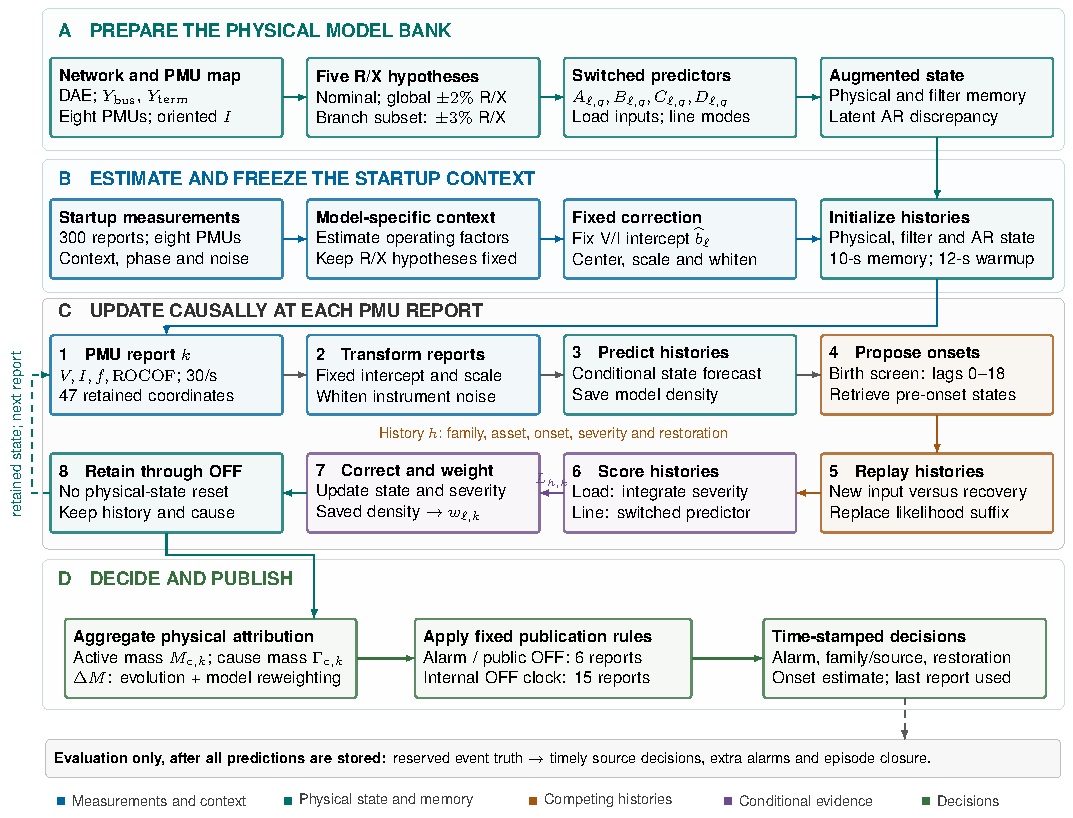
\includegraphics[width=.98\textwidth]{figures/generated/narrative_architecture.pdf}
\caption{Implemented physical inference in four stages. (A) Construct switched network and PMU predictors. (B) Estimate the startup context and fix its observation correction. (C) Compare new intervention histories with retained recovery at each report, using stored pre-onset states. (D) Aggregate attribution and publish qualified alarm, source and restoration decisions. The public six-report rules and the internal 15-report OFF clock are distinct; their support conditions are specified in Section~\ref{sec:narrative-method}. Dashed feedback retains state for the next report. Reserved truth enters only the later evaluation.}
\label{fig:joint-architecture}\end{figure*}

Physical restoration does not erase machine motion. A flat reference can
mislabel its remaining oscillation as a second event; suppressing all alarms
during recovery can hide an actual second event. A corrected voltage offset
also need not correct the response to a later input.

DAE estimators recover unmeasured electrical states
\cite{katanic2024recursive}; outage detectors compare physical hypotheses
\cite{chen2016quickest,rovatsos2017outage}; and simulated trajectories
support sparse-PMU fault diagnosis \cite{warner2023highfidelity}. These
ingredients are established. Our question is whether a continuing recovery
should explain a new PMU change or yield to a later intervention hypothesis.

We formulate a causal attribution procedure that keeps the estimated
physical response after an intervention ends and tests subsequent changes
against that continuing response. The paper makes three bounded contributions:
\begin{enumerate}
\item It specifies an executable physical measurement contract in which a
switched DAE and oriented terminal map generate the candidate PMU paths.
\item It evaluates a continuous history bank that compares new load or line
interventions with retained recovery, integrates local load severity, and
reports active mass $M$ separately from originating-cause mass $\Gamma$.
These are summaries of an approximate, screened hypothesis bank.
\item It measures timely family/source attribution, unmatched alarms and
restoration behavior on a prespecified catalog, and states exactly how that
evidence differs from two frozen ExtraTrees procedures and historical
window-based results.
\end{enumerate}
The complete physical bank attributes
\ReaderPhysicalLoad{}/\ReaderFamilyTotal{} load realizations before OFF
versus \ReaderETLoad{}/\ReaderFamilyTotal{} for the causal ExtraTrees
reference. Under out-of-bank R/X it raises \ReaderPhysicalOutsideExtras{}
versus \ReaderETOutsideExtras{} unmatched alarms. Thus the supported gain
is timely load attribution with a larger alarm burden. A separate posthoc component study tests amplitude-evidence scoring and
physical-state carry at inferred closure. It is not an independent confirmation
and cannot establish a benefit until all four arms and their intervals are
reviewed.

The test uses nine candidate load buses and nine lines in a fixed IEEE-39
simulation. It does not establish an all-family hackathon score, calibrated
event probabilities or real-time deployment.

\section{Related Work}
\label{sec:narrative-related}

DAE and unknown-input estimators recover hidden states or inputs
\cite{gillijns2007input,nugroho2022dae,katanic2024recursive}; functional
observability and diagnosability ask which states or sources can be
distinguished \cite{fernando2010functional,montanari2022functional,
eriksson2013diagnosability,scharf1994matched}. Physical outage inference
already uses network hypotheses, uncertain states and sequential tests
\cite{tate2008outage,zhao2014outages,chen2016quickest,
rovatsos2017outage}. Sparse input recovery estimates forcing locations
and unknown initial states in linear dynamics \cite{anguluri2023group}.
Sensor placement limits the information available at remote PMUs
\cite{jamei2020limits,conte2023fault,yildiz2025sparse}.

Warner \emph{et al.} compare simulated voltage/current paths across an
unknown-onset window for short-circuit line identification
\cite{warner2023highfidelity}. Yang, Chen and Zhai combine partial-PMU
algebraic measurements with particle-filter estimates of generator dynamic
states, then monitor outage signatures with an EWMA on the IEEE-39 system
\cite{yang2021particle}. This is a close physical precedent for line
outage detection; the present evaluation instead attributes load and line
interventions through OFF and successive recovery. Neither study is run as a
same-data benchmark here. Multiple-model filters and adaptive history banks
already retain conditional modes \cite{blom1988imm,boers2005m3h}; sequential
diagnosis has established error/delay theory under specified observation
laws \cite{warner2024matrix}. Our screened, pruned bank inherits none of
those general optimality or delay guarantees.

Learned PMU classifiers and physical uncertainty models provide other
routes \cite{pandey2020realtime,li2024knowledge,yildiz2024few,
ensaf2023kernel,tartakovsky2023gp,albustami2026dae,nagi2022trajectory}.
For example, Li \emph{et al.} embed disturbance-type/topology and
localization-cost constraints in a spatiotemporal graph-convolutional
model \cite{li2024knowledge}. Our physical route instead computes the
observation likelihood of candidate interventions; its graph is the
admittance network and terminal map, not a learned message-passing layer.
The two frozen ExtraTrees implementations test supervised references,
not all learned diagnosis. The new contribution claimed here is the
specified sparse-PMU procedure and its evidence: new interventions and
retained recovery histories compete for the same causal reports, with
component experiments explaining the role and limits of physical
representation. We do not claim that combining physics, Bayes and a
tensor is itself new. Table~\ref{tab:literature-capability} distinguishes the
neighboring tasks and the comparators actually executed here.

\begin{table*}[t]\centering\small
\caption{Closest inference contracts. Chen and the two fixed ExtraTrees
adapters are the executed comparators. An untested capability is not an
algorithmic impossibility.}
\label{tab:literature-capability}
\begin{tabularx}{\textwidth}{@{}lXXX@{}}\toprule
Route & Mechanism & Evaluated target & Role in this study\\\midrule
Chen / Rovatsos & Network likelihoods and sequential tests & Line outages; Rovatsos includes transients & Chen on persistent-line first decisions\\
Warner high-fidelity & Simulated V/I paths and onset search & Short-circuit line candidates & Closest trajectory precedent; no common-data run\\
Yang--Chen--Zhai (2021) & Particle filter for generator states; EWMA outage monitoring & Line-outage detection with partial PMUs on IEEE-39 & Closely related line detector; no continuous load/restoration comparison\\
Adaptive Matrix CuSum & Sequential diagnosis with error/delay analysis & One unknown distributional change & Statistical precedent; no inherited guarantee\\
DAE / stochastic-state estimation & Physical state and uncertainty models & States, unknown inputs or parameters & Components and adjacent tasks\\
Learned PMU diagnosis & Features or constrained representations & Event families and locations & Two frozen ExtraTrees references\\
Physical history bank here & Estimated-past-state paths and recovery & Successive catalog load/line events & Timely attribution, extras and restoration\\\bottomrule
\end{tabularx}\end{table*}

\section{Problem and Measurement Model}
\label{sec:narrative-problem}

At report $k$, inference uses measurements through $t_k=k/30$ to decide
whether a physical intervention occurred. Detection concerns its presence;
classification selects a physical operator; localization selects a bus or
branch. These outputs can become reliable at different times. We record
the estimated physical onset $\widehat\tau$ separately from the alarm and
diagnosis emission times.

Figure~\ref{fig:reference-event-types} introduces the broader measurement
phenomena using the reference record released with the SGSMA 2026
competition. Faults, line changes,
generation changes and load changes alter the physical network; missing or
corrupted reports alter observation integrity. The causal attribution test
addresses load changes and line openings with restoration; missing and
corrupted data are diagnosed by the integrity relations of
the supplementary integrity analysis. Faults and generation changes provide
context, not additional validated event classes.

\begin{figure*}[t]\centering
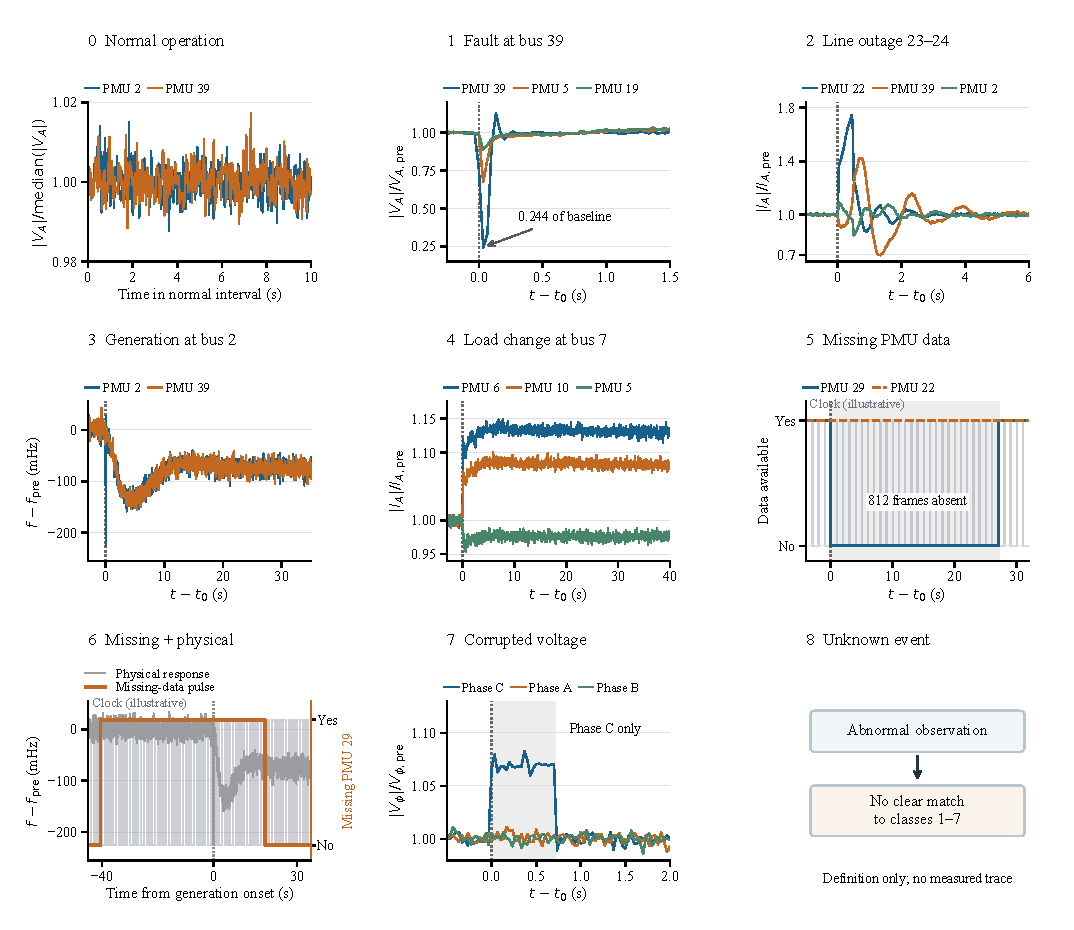
\includegraphics[width=.98\textwidth]{figures/generated/event_taxonomy_grid.pdf}
\caption{Representative signatures from the archived RAW0001 reference simulation of the SGSMA 2026 competition, arranged by label 0--8. Class 0 shows a normal interval; classes 1--5 and 7 retain the original trace values. Class 6 applies an illustrative data-loss mask from 0 to 30 s to the PMU 2 frequency trace (generation onset at 15 s): orange shows the available response and Yes level; blue marks No, while gray shows the response hidden during the gap, not a detector reconstruction. The mask is not the recorded outage interval. The gray clock trains in panels 5 and 6 are illustrative, not measured report timing. Class 8 is a definition schematic, not an observed trace or a validated bank output. Event traces are aligned to source labels for illustration only. Only load and line mechanisms enter the main causal evaluation.}
\label{fig:reference-event-types}\end{figure*}

The network has 39 buses, but the prescribed PMU set is
\begin{equation}
 \mathcal P=\{2,5,6,10,19,22,29,39\}.
 \label{eq:narrative-pmus}
\end{equation}
Voltage is measured at each PMU bus. Current is measured at a specified branch terminal, which can differ from that bus. The causal implementation uses 47 coordinates: eight voltage magnitudes, eight voltage angles, eight current magnitudes, seven current angles, eight absolute frequencies and eight ROCOFs, at 30 reports/s. BUS39 current angle is excluded because its interpretation remains partially validated. The BUS5 current terminal retains the provisional historical 5--6 assignment. These are declared measurement assumptions, not identities inferred from classification accuracy.

The exported magnitudes are in V and A, angles in degrees, frequency in Hz
and ROCOF in Hz/s. Internal centered coordinates do not replace the
definition of absolute frequency. These are reporting-rate phasor measurements;
waveform harmonics or THD are not measured by these channels.

The causal stream is exported from one balanced complex phasor per PMU:
phase A supplies the voltage and current magnitudes and angles. The CSV
exporter constructs B and C by equal magnitudes and angle offsets of
$-120^\circ$ and $+120^\circ$. Retaining A therefore loses no independent
phase information in these synthetic records; it is not measured
positive-sequence extraction or a model of unbalanced faults. The vector is
$y_k=(|V_A|_{\mathcal P},\angle V_A{}_{\mathcal P},
|I_A|_{\mathcal P},\angle I_A{}_{\mathcal P\setminus\{39\}},
f_{\mathcal P},\dot f_{\mathcal P})_k$.
The supplementary measurement table gives all eight current-terminal
assignments, polarities, gains and phase offsets. Products of voltage and
current measured at different terminals are power proxies.

% PROTECTED FIGURE: retain this single-column IEEE-39 diagram. See AGENTS.md.
\begin{figure}[t]\centering
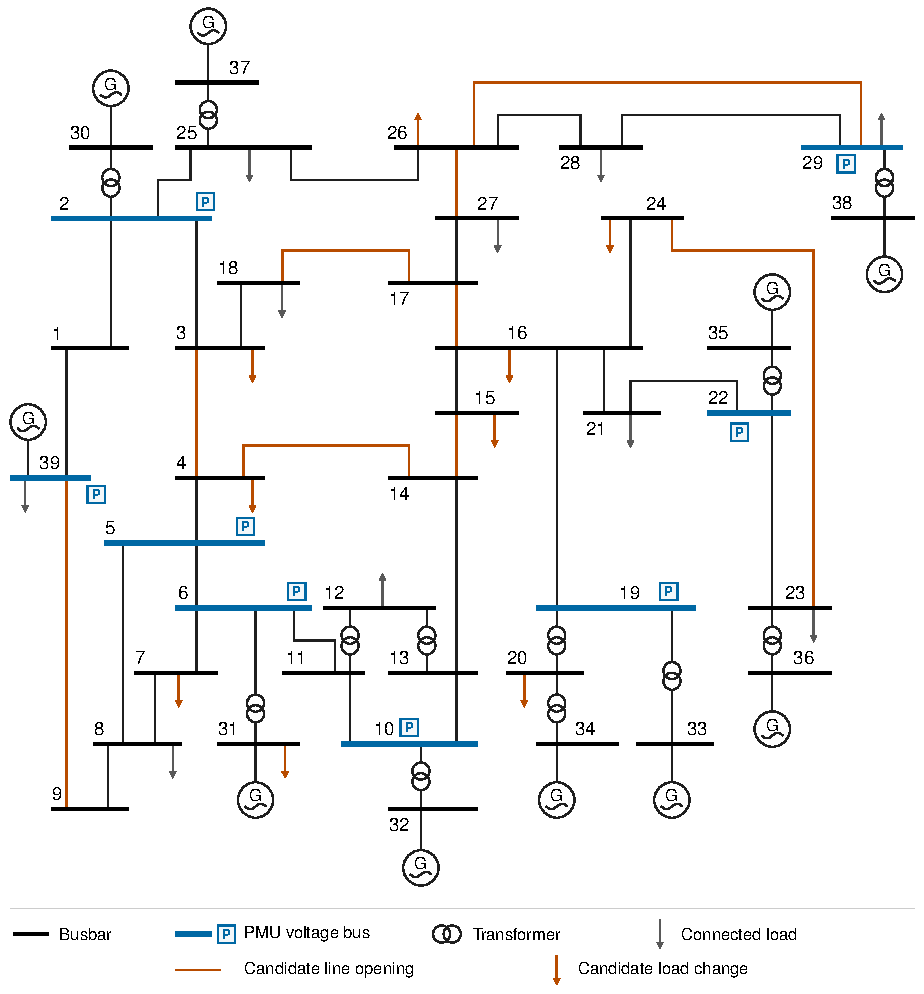
\includegraphics[width=\columnwidth]{figures/generated/narrative_topology.pdf}
\caption{IEEE 39-bus single-line diagram: 46 branches, 12 transformers and 10 generators. Blue bars and P marks locate the eight voltage PMUs. Orange branches and load arrows identify the nine line and nine load candidates; gray arrows denote other loads. Current terminals follow the separate measurement contract.}
\label{fig:narrative-topology}\end{figure}

The physical model is
\begin{align}
 \dot x&=f_q(x,z,u;\theta),&0&=g_q(x,z,u;\theta),\label{eq:narrative-dae}\\
 h_k&=H_q(x_k,z_k,u_k),\nonumber\\
 \eta_k&=F_M(\eta_{k-1},h_k;\theta_M),\nonumber\\
 y_k&=G_M(\eta_k,h_k;\theta_M)+b+\varepsilon_k.\label{eq:narrative-measurement}
\end{align}
Figure~\ref{fig:physical-measurement-chain} maps these physical and
measurement operations to the report consumed by inference.
\begin{figure*}[t]\centering
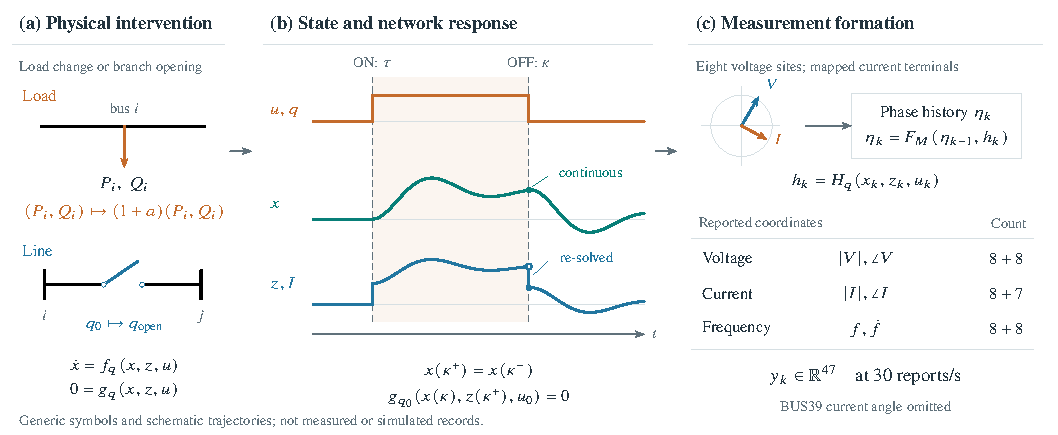
\includegraphics[width=.99\textwidth]{figures/generated/physics_measurement_chain.pdf}
\caption{Illustrative chain from load/line intervention to causal PMU report.
At OFF, the operator returns to baseline while $x$ and phase-history $\eta$
persist; algebraic voltages and currents are re-solved. Eight PMUs yield 47
coordinates at 30 reports/s; BUS39 current angle is omitted. Symbols and traces
are schematic. Phase B/C are reconstructed from A; raw waveforms and harmonics
are not inference inputs.}
\label{fig:physical-measurement-chain}\end{figure*}
Here $x$ contains machine and control dynamics, $z$ the algebraic network
variables, $q$ the topology/intervention mode, and $\theta_M$ the measurement
convention. $H_q$ selects electrical phasors; $\eta_k$ retains the causal
phase history used for frequency/ROCOF and the measurement-filter state.
The observation thus depends on an augmented state. Bus frequency comes
from phase evolution, not a machine's rotor speed. Instrumental noise is
generated by the noise model described in Section~\ref{sec:narrative-protocol}.

An intervention history is the discrete tuple
$h=(e,c,\tau,\kappa,\mathcal I)$: family, source, onset, restoration time
($\kappa=\infty$ for a sustained event) and, for a load, a severity interval
$\mathcal I$. The severity $a\in\mathcal I$ is a continuous latent variable
conditioned on $h$ and integrated in the evidence; a line opening has no
severity. A load changes its local P/Q setpoints by the common factor
$1+a$; a line opening switches its branch primitive. For the
supported impulse-free switches,
\begin{equation}
 x(\tau^+)=x(\tau^-),\qquad g_{q^+}(x(\tau^-),z(\tau^+),u;\theta)=0.
 \label{eq:narrative-switch}
\end{equation}
The algebraic voltage/current response may jump even though dynamic states remain continuous. Physical restoration reverses the intervention operator. It does not return the machines to their pre-event state, so electrical recovery can continue after OFF.

Switch-aligned reports use the consistent post-switch algebraic solution.
The local reduction requires an invertible algebraic Jacobian after fixing
the angle reference; the catalog excludes islanding line alternatives.
Successful solves and local residual checks validate the admitted cases,
not global regularity for arbitrary switching topologies.

\begin{table}[t]\centering\small
\caption{Scope of the executed causal component. The source is an intervention asset; it is not necessarily a measured PMU bus.}\label{tab:narrative-scope}
\begin{tabularx}{\columnwidth}{@{}lXX@{}}\toprule
Case & Physical operator & Executed claim\\\midrule
Normal & No intervention & Monitor after startup\\
Load & Local P/Q factor; optional restoration & Nine candidate buses\\
Line & Branch open; optional reclose & Nine candidate branches\\
Fault/generation & Different shunt/input/trip operators & Outside this causal test\\
Missing/bad data & Measurement-integrity mechanism & Parity diagnosis (supplement)\\
Unknown & Unresolved diagnosis & Not a new physical family\\\bottomrule
\end{tabularx}\end{table}

The generator stores event schedules and true states separately from the PMU stream. Inference receives the nominal network, permitted calibration and reports through the current time. It receives no source, switch time, true R/X realization or solver state. Initial operating context and noise scale are estimated from 300 startup reports; monitoring begins after a 12-s warmup. This startup estimate assumes an intervention-free prefix.

\section{Recovery-Aware Physical Attribution}
\label{sec:narrative-method}

Figure~\ref{fig:joint-architecture} gives the report-level logic. A
history is a proposed cause and trajectory, not just a bus label. The
inference bank predicts the next report under no new event, a new load or
line action, or retained recovery. Its switched predictors come from the
network DAE and oriented PMU terminal map. Statistical filtering handles
uncertain states and residual error. The nonlinear simulator generates the
observations; inference uses local predictors, not a new full simulation
for every hypothesis and report.

\subsection{Construct the Predictor From the Network}

Kirchhoff constraints and complex power connect sources to remote PMUs:
\begin{equation}
 I_{\rm bus}=Y_{\rm bus}V,\quad
 I_{{\rm term},r}=Y_{{\rm term},r}V,\quad S_i=V_i I_{{\rm bus},i}^{*}.
 \label{eq:narrative-electrical}
\end{equation}
Terminal rows retain orientation, line charging and transformer ratios.
A measured terminal current is not a nodal injection. A line opening
changes the branch stamp and therefore the algebraic voltages and measured
currents. A terminal map changes directly only if the switched branch is
itself measured; none of the nine tested line candidates is a measured PMU
terminal. The load operator scales both $P_{\rm set}$ and $Q_{\rm set}$
by $1+a$ with the fixed constant-impedance ZIP fractions, while the line
operator switches the selected branch between active and open modes.

The executed plant has 114 differential states, 78 algebraic variables
and 38 load-input coordinates. Its ten Sauer--Pai machines use AVR Type I
with quadratic ceiling and TGOV1 governors, except the bus-39 machine,
which has no external governor or excitation-control inputs. All 19 load
models use constant-impedance ZIP fractions. With injection sign convention,
\begin{equation}
 P_i=(1+a_i)P_i^0\left|V_i/V_{{\rm set},i}\right|^2,\qquad
 Q_i=(1+a_i)Q_i^0\left|V_i/V_{{\rm set},i}\right|^2.
 \label{eq:implemented-load-law}
\end{equation}
Here $P_i^0<0$ represents consumption; reactive injection can be positive
for a capacitive load. The archived equilibrium and voltage setpoints,
including those at buses 31 and 39, define the executed operating point.

On a regular index-one DAE chart with a fixed angle reference,
\begin{align}
 \delta z&=-g_z^{-1}(g_x\delta x+g_u\delta u),\nonumber\\
 \delta\dot x&=A_q^{\rm red}\delta x+B_q^{\rm red}\delta u,\nonumber\\
 A_q^{\rm red}&=f_x-f_zg_z^{-1}g_x,\quad
 B_q^{\rm red}=f_u-f_zg_z^{-1}g_u.
 \label{eq:narrative-reduction}
\end{align}
For the instantaneous electrical observation map $H_q(x,z,u)$, the
corresponding output operators are
\begin{equation}
 C_q^{\rm red}=H_x-H_zg_z^{-1}g_x,\qquad
 D_q^{\rm red}=H_u-H_zg_z^{-1}g_u.
 \label{eq:electrical-output-reduction}
\end{equation}
They propagate a perturbation at an unmeasured source to the selected
voltage and oriented-current channels. Network connectivity enters through
the branch stamps in $g_q$ and, where applicable, $H_q$; eliminating unmeasured algebraic
variables generally produces dense reduced operators. The graph therefore
constrains the prediction without a learned graph embedding. A changed
terminal operator would also contribute directly through $H_q$; the
tested line modes keep the same terminal map. The implementation discretizes the admitted
switch modes and adds causal phase-history operators for frequency and
ROCOF. The generator estimates phase derivatives with a robust,
magnitude-weighted quadratic fit over 21 reports. The predictor approximates
that operation with a fixed unweighted quadratic fit over the same history;
these operators need not agree when weights change. Inertia, controls and
load law remain those of the fixed plant.

After augmenting instrumental memory, a conditional predictor has the
local form
\begin{align}
 \xi_{k+1}&=A_{\ell,q}\xi_k+b_{\ell,q}+B_{\ell,q}a+w_k,\nonumber\\
 r_k&=C_{\ell,q}\xi_k+d_{\ell,q}+D_{\ell,q}a+v_k.
 \label{eq:implemented-predictor}
\end{align}
Here $r_k$ contains reference-corrected, scaled and instrument-whitened PMU coordinates, $\ell$ is a fixed
network hypothesis, and $\xi_k$ contains physical deviation states, phase
history and predicted measurement-filter memory. Observed colored-instrument
filters whiten measurements; their corresponding predictor memory is
deterministic. Additional latent AR states represent persistent discrepancy,
with preset quiet/load/line/recovery covariance and drift regimes. This
statistical discrepancy model is distinct from the plant equations.
$v_k$ denotes the remaining innovation. A load has scalar severity within
its specified P/Q direction. A line uses a switched operator rather than
a fictitious load-amplitude fit. Equation~\eqref{eq:implemented-predictor} states the generic local model;
the implemented update combines propagation and observation into an
operator on the previous state. The supplement gives that indexing and
the associated transition gain explicitly. States from different equilibria are not
interpreted as an absolute rotor-state mixture.

\subsection{Estimate Context From the Startup Prefix}

Each network hypothesis uses the same 300 startup reports to estimate
operating factors, reference phase and noise scale. Voltage/current
coordinates receive a constant discrepancy correction,
\begin{equation}
 \widehat b_\ell=\overline y_{0:299}-y_\ell^{\rm ref},
 \qquad b_{\ell,k}=\widehat b_\ell\quad(k\ge300).
 \label{eq:continuous-intercept}
\end{equation}
Angular differences respect wrapping and the common reference. Frequency
and ROCOF use empirical prefix centers. The correction remains fixed so it
cannot track a later load step and subtract its signature. This estimates
an observation discrepancy, not the true impedances. Prefix estimates
enter by substitution rather than through a full joint parameter posterior.

\subsection{Compare Unknown-Onset Histories}

The method retains ten seconds of past conditional states. Its frozen birth screen proposes selected onsets at 19 candidate lags,
0--18, within a 20-report candidate window. It does not enumerate every
onset in the 300-report history.
Each history specifies family, asset, onset,
restoration mode and severity. It starts from the stored conditional state
before its proposed onset. That state already contains any ongoing
recovery; an alarm does not reset the predictor to equilibrium.

For a retained load history, conditional Gaussian filtering yields a
residual $e$, severity response $s$ and covariance $S$. Unknown severity
has a truncated-Gaussian distribution inherited from previous reports:
\begin{equation}
 L_{h,k}=\int_l^u \mathcal N(e;sa,S)
             \operatorname{TN}_{[l,u]}(a;\mu,v)\,da.
 \label{eq:narrative-evidence}
\end{equation}
The supplement derives the closed form by completing the square and
works through a numerical example. It also specifies the conditional
state representation $m_h+d_h a$ and its update. The local amplitude
integral is exact for the stated conditional Gaussian model. The complete
bank remains approximate: regime covariances are shared from
nominal-operator Riccati equations, context estimates enter by substitution,
and histories are screened and pruned. At episode closure the augmented
state mixture mean is retained and omitted between-history spread is recorded.
A fully Bayesian posterior over states, context and all histories is not claimed.

The rolling screen proposes histories; it is not another independent
observation. Replaying a suffix replaces its original no-new-event suffix
likelihood. The sequential update therefore counts each report once,
rather than repeatedly accumulating overlapping ten-second windows.

Within each fixed network hypothesis $\ell$, let $\mathcal H_{\ell,k}$
denote its screened non-null histories and
$\mathcal A_{\ell,k}=\mathcal H_{\ell,k}\cup\{0\}$ include the
null history $0$ (no intervention). For each currently admitted candidate
$h$, let $\bar\pi_{\ell,h,k}$ denote its predicted mass before scoring the
current report. For an existing history this prediction applies the
implementation's OFF hazards to survivors and children, generated on demand.
For a proposed birth at report $\tau$, it includes the null-parent mass,
the frozen birth prior, and the replay likelihood ratio
$\exp(\ell^{\rm new}_{\tau:k-1}-\ell^{\rm old}_{\tau:k-1})$ with the
corresponding transition and prior terms. Thus the proposal replaces the
old no-event suffix before the current report is scored; the reports in the
replayed suffix are not counted twice. The supplement gives the corresponding score identity. The report update and within-hypothesis
normalization are
\begin{align}
\widetilde\pi_{\ell,h,k}&=L_{\ell,h,k}\bar\pi_{\ell,h,k},\qquad
\widetilde\pi_{\ell,0,k}=L_{\ell,0,k}\bar\pi_{\ell,0,k},\nonumber\\
\pi_{\ell,h,k}&=\frac{\widetilde\pi_{\ell,h,k}}
 {\sum_{j\in\mathcal A_{\ell,k}}\widetilde\pi_{\ell,j,k}}.
\label{eq:history-mass-update}
\end{align}
This is a normalization scheme for the currently admitted candidates, not
a full Markov transition over all possible histories. After each update, the
screen and beam prune hypotheses and the retained masses are renormalized
jointly with the null. The outer weights $w_{\ell,k}$ are updated from
network-level predictive densities and combine these conditional masses in
$M$ and $\Gamma$; they are not part of the within-bank normalizer. The
resulting masses do not define a calibrated posterior.

\begin{figure*}[t]\centering
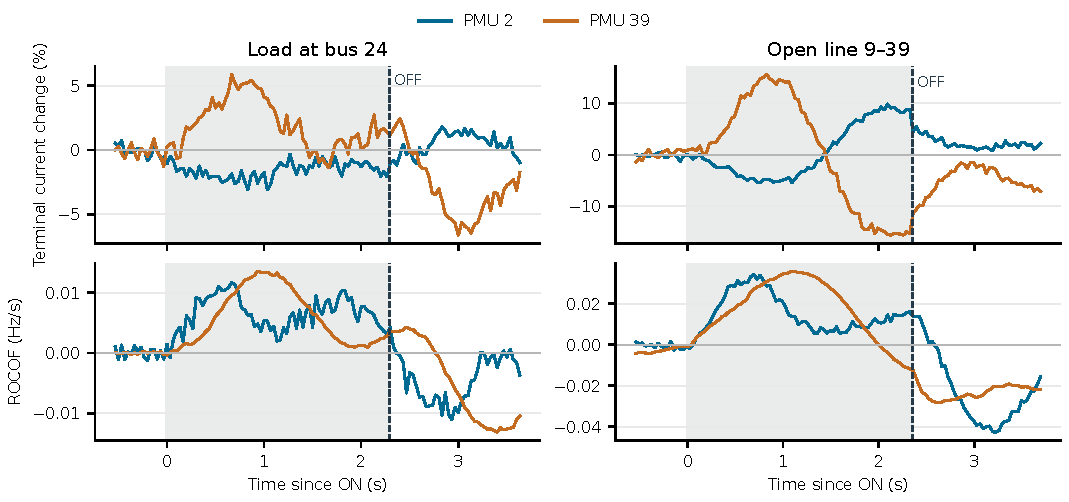
\includegraphics[width=.91\textwidth]{figures/generated/reader_observed_signals.pdf}
\caption{Two interventions from one continuous development record. Current change and ROCOF at PMUs 2 and 39 remain dynamic after physical OFF (dashed line). The gray interval is the true active period, shown only for explanation; inference uses all eight PMUs without event timing. These two PMUs illustrate the traces and were fixed for both panels.}
\label{fig:narrative-signals}\end{figure*}

\subsection{Represent Fixed Network Uncertainty}

The bank contains nominal, global $\pm2\%$, and selected-branch $\pm3\%$
paired R/X hypotheses. Parameters stay constant within a hypothesis. Its
outer weight uses a predictive density formed before the current-report
state update and proposal selection:
\begin{equation}
 w_{\ell,k}=\frac{w_{\ell,k-1}p_\ell(y_k\mid\mathcal F_{k-1},\widehat b_\ell)}
 {\sum_jw_{j,k-1}p_j(y_k\mid\mathcal F_{k-1},\widehat b_j)}.
 \label{eq:continuous-weights}
\end{equation}
Startup-fitting reports are not scored again as independent model-selection
evidence. The mixture covers a finite set of network alternatives rather
than identifying a continuous impedance posterior.

\subsection{Keep Recovery as a Competing Physical Explanation}

Restoring an input or topology at $\kappa$ does not restore the pre-event
state: $x(\kappa^+)=x(\kappa^-)$. On a regular local post-restoration chart,
the difference from a same-context no-new-intervention trajectory obeys
\begin{align}
 \delta x_h(t)&\simeq\Phi_0(t,\kappa)\delta x_h(\kappa),\nonumber\\
 \delta y_h^{\rm net}(t)&\simeq C_0(t)\Phi_0(t,\kappa)\delta x_h(\kappa),
 \quad t>\kappa.
 \label{eq:recovery-response}
\end{align}
Here $y^{\rm net}$ denotes voltage/current coordinates before the instrument map.
Instrumental memory is retained as well. This local interpretation of known
dynamics explains why the reference after OFF is a trajectory, not a zero
residual; it is not a new propagation theorem.

For conditional history mass $\pi_{\ell,h,k}$, define active and
originating-cause masses for an admissible family/source cell $c$:
\begin{align}
 M_{c,k}&=\sum_\ell w_{\ell,k}\sum_{h:c(h)=c}
       \pi_{\ell,h,k}\,\mathbf1\{h\text{ active at }k\},\nonumber\\
 \Gamma_{c,k}&=\sum_\ell w_{\ell,k}\sum_{h:c(h)=c}\pi_{\ell,h,k}.
 \label{eq:active-cause-masses}
\end{align}
A retained history can stop being active while its cause still explains
recovery. Later interventions compete with those histories. The
implementation stores 18 admissible cells, not every family at every bus.
After confirmed episode closure, explicit histories are compressed into
the retained state mean. Cause masses describe the current bank, not a
permanent ledger of all past interventions.

Writing the conditional active mass as $M_{\ell,c,k}$ yields
\begin{align}
 \Delta M_{c,k}&=\sum_\ell w_{\ell,k}
               (M_{\ell,c,k}-M_{\ell,c,k-1})\nonumber\\
 &\quad+\sum_\ell(w_{\ell,k}-w_{\ell,k-1})M_{\ell,c,k-1}.
 \label{eq:continuous-delta}
\end{align}
The terms distinguish within-model evolution from model reweighting.
This accounting identity aids interpretation, without constituting a new
tensor factorization. The masses are approximate attribution weights;
probability calibration and globally optimal filtering are not established.

\subsection{Emit Separate Detection, Diagnosis and Restoration Messages}

The internal observer proposes an alarm after the six-report persistence
rule above the 0.99 active-mass threshold. Public alarm publication additionally requires an
internal pending episode and six reports of qualified active support:
the frozen source screen qualifies load cells, while admitted line cells
qualify through their switched operator. Public OFF requires six reports
above 0.99 for the diagnosed cell's joint cause-and-restoration mass.
The observer also has a separate, more conservative 15-report internal
OFF clock. Diagnosis selects the family with greatest summed cause mass and then
the highest-mass source within that family. It is emitted after six
reports of stable cause support or at the 15-report post-alarm deadline.
The supplement defines the source screen, early line rule and episode
replacement, including how internal messages are propagated publicly. Every message records emission time and
the last report used. A diagnosis can be correct eventually but too late
to precede physical OFF.

The nominal comparator uses the same nominal conditional model with its
own fixed publication path. Comparing nominal and mixture evaluates two
complete configured procedures; it does not isolate the outer network bank
from publication decisions. The admission-rule ablation tests a different publication
decision; it is not a pure recovery-memory ablation.

The supplement records the frozen birth/restoration hazards, severity
prior and integration intervals, restoration-child rules and beam limits,
together with the execution sequence and illustrative calculations.
These details preserve the archived configuration; the compact algorithm
below states the report order and information boundary.

\subsection{Per-Report Algorithm and Computational Boundary}

\noindent\textbf{Algorithm 1: one causal update.}
Input: nominal model, fixed method configuration and PMU reports.
Initialize context, reference, noise and conditional states from the 300
startup reports. Event truth is never an input.
\begin{enumerate}
\item Transform report $k$; predict it from each retained physical or
recovery history. Save each network model's predictive density before
screening or correcting with this report.
\item Screen 19 candidate onset lags (0--18) within the 20-report window. Start each proposed history
from its stored pre-onset state and replay its suffix, replacing the old
suffix likelihood once.
\item Score histories, integrating load severity or using the switched
line operator. Then correct state and severity, update network weights,
and prune by the fixed rules. Retain state and cause through restoration.
\item Aggregate active mass $M$, cause mass $\Gamma$ and $\Delta M$.
Apply the frozen alarm, source and OFF rules; record emission time,
estimated onset and last report used.
\end{enumerate}
The nonlinear simulator constructs observations; this algorithm propagates
local switched predictors. The input grid is 30 reports/s. Causality
concerns report availability; acquisition throughput, computation time
and the electrical history needed for a decision are separate quantities.
Wall-clock real-time operation has not been established.

\FloatBarrier
\section{What Physical Structure and Learned Features Recover}
\label{sec:evidence-bridge}

The continuous estimator builds on three distinct questions: what can be
reconstructed at unmeasured buses, what response distinguishes candidate
sources, and how evidence should be assigned when several explanations
fit. The following component experiments answer parts of these questions.
They use different cohorts and are not ablations of the final continuous
estimator. Figure~\ref{fig:evidence-bridge} places their measured effects
side by side without pooling their scores.

\begin{figure*}[t]\centering
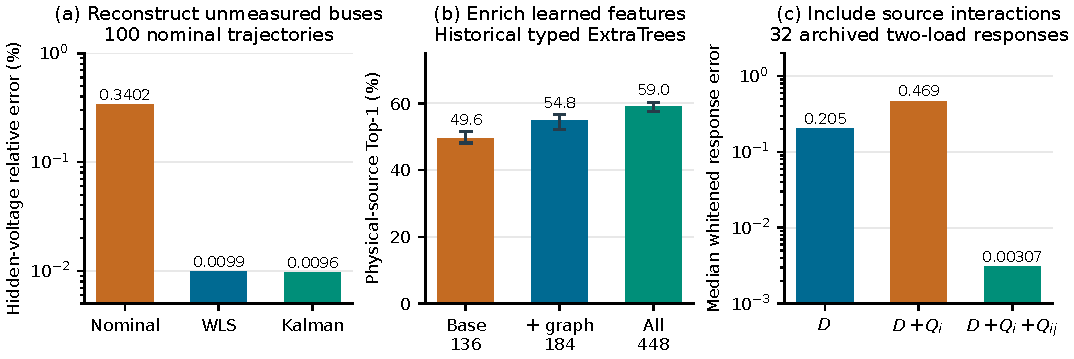
\includegraphics[width=.99\textwidth]{figures/generated/evidence_bridge.pdf}
\caption{Three separate component experiments. (a) Mean relative error of
the 31 unmeasured bus voltages under a matched nominal model; this is not a
PMU compliance TVE test. (b) Mean physical-source Top-1 over three model
seeds, each scored on 7,915 labeled physical samples, in the historical
typed-ExtraTrees feature study; whiskers show the
seed range, not a confidence interval. These 136--448-feature models are
neither the final hackathon submission nor the causal comparators.
(c) Median whitened prediction error at the archived 120-report horizon
for two-load responses: mixed-source terms matter, while adding only
self-curvature worsens this metric. Each panel has its own units and cohort.}
\label{fig:evidence-bridge}\end{figure*}

\subsection{Recovering Unmeasured Voltages Is Not Yet Event Attribution}
In 100 nominal test trajectories, the mean hidden-voltage relative error
falls from \BridgeNominalError\% for the equilibrium reference to
\BridgeWLSError\% for snapshot weighted least squares and
\BridgeKalmanError\% for a causal Kalman reconstructor. Most of this
improvement comes from conditioning the physical network on the measured
phasors; temporal filtering adds a smaller improvement. This supports
reconstruction under that model and sensor placement, not unique recovery
of every source. The independently evaluated Kalman reconstructor is not
silently substituted for the conditional observer in Fig.~\ref{fig:joint-architecture}.

\subsection{Physical Features Remain a Useful Learned Route}
The historical feature study raises physical-source Top-1 from
\BridgeBaseTop\% with 136 features to \BridgeGraphTop\% with graph-temporal
features added, and \BridgeFullTop\% with the full 448-feature set.
Voltage level, relative angle, frequency, time scale and spatial coherence
carry complementary information; Fig.~\ref{fig:evidence-bridge}(b) reports
an executed feature comparison rather than an inferred explanation of
tree importance. Electrical features make a classifier physics-informed
in its representation. They do not enforce Kirchhoff balance on its
predicted label or compute the PMU response of a candidate intervention.

For phase-to-neutral RMS phasors and a declared current orientation,
\begin{equation}
 S_{ij}=P_{ij}+\mathrm jQ_{ij}
       =\sum_{\phi\in\{a,b,c\}}V_{i\phi}I_{ij,\phi}^{*}.
 \label{eq:bridge-terminal-power}
\end{equation}
This expression requires voltage and current at the same terminal.
In the frozen map, the bus-2 voltage is paired with a current measured at
bus 3, and the bus-10 voltage with a current at bus 11. Their raw channel
products are therefore power proxies, not exact terminal powers. Even a
co-located terminal power is not the bus's net injection unless all
relevant terminals are accounted for. Frequency and ROCOF complement the phasors
but share the instrument's angle processing; the likelihood must account
for that dependence. Fundamental-frequency phasors also do not determine
harmonic distortion. Thus adding nominally physical features does not
by itself supply missing harmonic or nodal-injection measurements.

\subsection{Mixed-Source Response Coefficients}
For simultaneous load changes, a second-order response approximation
includes products of the input amplitudes. In the archived two-load
experiment,
\begin{equation}
 s_{q,n}(a)=\sum_i D_{qni}a_i+\sum_i Q_{qni}a_i^2
               +\sum_{i<j}Q_{qnij}a_ia_j,
 \label{eq:bridge-response-tensor}
\end{equation}
where $q$ indexes PMU coordinates, $n$ elapsed reports and $i,j$ load
sources. Centered nonlinear simulations estimate the coefficients; the
$Q$ terms include their Taylor scaling. The mixed term represents the
interaction of two simultaneous load changes. Across 32 archived
two-source responses, median whitened error is \BridgeDError{} for $D$,
\BridgeQError{} after self-curvature, and \BridgeMixedError{} after mixed
terms. This is evidence for response fidelity in that local experiment.
It is not a measured classification gain from inserting this second-order
tensor into the continuous load/line bank, which uses switched local
predictors instead.

The coefficients in \eqref{eq:bridge-response-tensor} form a tensor over
measured coordinate, elapsed time and source indices. The useful term is
the physical cross-source interaction $Q_{qnij}$; the array's shape alone
does not provide an accuracy or computational advantage.
In the continuous estimator, $M$ is instead a vector of aggregated
source/family weights at each report, and $\Delta M$ is its temporal
difference, as defined in \eqref{eq:active-cause-masses}--\eqref{eq:continuous-delta}.
That implementation does not require a tensor decomposition or a
tensor-learning library.

\subsection{Why Integrate Severity Rather Than Select the Best Fit?}
An extra source with zero amplitude can reproduce a smaller source set.
Best-fit residual alone therefore cannot decide cardinality. In the
archived load-support estimator, the model-selection quantity is
\begin{equation}
 Z_S=\int p(r\mid s_S(a),\Sigma)p(a\mid S)\,da,
 \qquad p(S\mid r)\propto Z_Sp(S).
 \label{eq:bridge-batch-evidence}
\end{equation}
Integration accounts for the prior volume of amplitudes consistent with
the data, rather than rewarding only the best-fitting amplitude. This is
standard Bayesian model comparison applied to an electrical response
model, not a new Bayes rule. The archived implementation evaluates the
null, 16 single-source and 120 pair supports with 31-point Gauss--Hermite
quadrature per amplitude. Table~\ref{tab:archived-support-bridge} shows
both its successes and its loss of resolution for weak sources.

\begin{table}[t]\centering\small
\caption{Archived joint cardinality-and-support decisions. Onset, load
family and operating context are supplied. These are noise replays of
shared physical trajectories, not independent continuous detections.}
\label{tab:archived-support-bridge}
\begin{tabular}{@{}lrr@{}}\toprule
Amplitude regime & Replays & Joint support Top-1 \\\midrule
Finite / finite & 1,440 & 100.00\% \\
Moderate / moderate & 1,440 & 98.82\% \\
Weak / strong & 1,440 & 66.25\% \\
Weak / weak & 5,760 & 24.38\% \\
\bottomrule\end{tabular}

\end{table}

An audit found a one-source evidence normalization offset in this
archive: the implemented cardinality prior is proportional to
$(0.20,0.50/(2\pi),0.30)$ rather than the declared $(0.20,0.50,0.30)$.
The table preserves the executed results under that effective prior;
it does not validate calibrated posterior probabilities or a corrected
replay. The continuous estimator uses separate, independently checked
local evidence code. Consequently these component results motivate the
physical/Bayesian construction, but do not establish that adding Bayes
or tensor storage alone causes its final accuracy advantage.

\section{Experimental Design}
\label{sec:narrative-protocol}

The test asks whether one method can attribute six successive load or line
interventions in a continuous trajectory, including an intervention that
begins while the preceding response is still recovering. The plant is a
fixed Julia/PowerDynamics IEEE 39-bus research candidate. Each parent is
integrated once across all ON and OFF actions; differential states are not
reset. PMU reports are exported at 30 frames/s, independently of solver
steps. A switch-aligned report uses the post-switch algebraic value.
RAW0001 informed the simulator retrospectively and is not an independent
test record.

The sealed evaluation has 18 six-event continuous parents, 27 persistent
line-opening parents and 12 normal parents. Every parent is replayed under
matched R/X, an R/X change represented in the model bank and an R/X change
outside it. Two instrumental-noise scales give 171 physical trajectories
and 342 observed records. The 648 continuous event realizations repeat
108 interventions; the physical parent, rather than the PMU frame or
replay, is the uncertainty unit. The earlier development examples in
Fig.~\ref{fig:narrative-rolling} are not part of this sealed comparison.

\subsection{What the Feature Baseline Actually Does}
The hackathon submission was a hierarchical detector, event classifier
and typed localizer based on ExtraTrees. It summarized each 30-s PMU
window with voltage/current magnitude and angle statistics, frequency,
ROCOF, missingness, phase spread, approximate P/Q, rolling changes,
RLS/Kalman level innovations and graph-temporal differences. Its selected
bundle reports 45,162 input features and internal simulated-validation
macro-F1 0.960 with exact localization 0.852. These numbers describe that
archive's broader nine-label, window-level task; they are not scores on
the present event-level cohort. The original submission is preserved.

To compare at 30 reports/s, an earlier development campaign built two
\emph{new}, frozen causal ExtraTrees adapters from 47 PMU coordinates.
Each coordinate is centered and robustly scaled using the quiet prefix.
For trailing windows of 1, 5 and 10\,s, the reference adapter computes
median, standard deviation, 10th/90th percentiles, a recent-quarter
change and RMS first difference. This gives $47\times3\times6=846$
features per report. The short-window adapter adds the current value and
mean, standard deviation and two lag changes at 3, 8 and 15 reports,
giving 1,457 features in total. Both use 400 trees, balanced class weights,
19 classes (quiet plus 18 assets), and six-report confirmation; tree votes
are scores, not calibrated event probabilities. Their training parents
precede and are disjoint from the sealed cohort. Neither model was
retrained or threshold-adjusted on these outcomes. The original split contains 32 local physical IDs for fitting (64
records, 78,784 training rows) and eight for validation (16 records).
A later dependency audit maps these to 26 fitting and eight validation
groups, with two normal-control groups shared across those sets. This
limits independence of the internal validation; it is not evidence of
leakage into the separate confirmatory cohort. The reference and
short-window classifiers already obtain only 0/72 and 4/72 timely load
attributions in that development validation. Their frozen performance
therefore does not represent a successfully optimized load classifier.

A later grouped retraining study uses 31 fit, eight validation and 17
reserved physical groups: approximately 70/30 development/reserved,
with an inner validation partition. That model is a separate artifact,
not either comparator executed in the confirmatory study. Randomly
splitting PMU reports 70/30 would allow correlated trajectories to cross
partitions. RAW0001 is a known retrospective transfer check, not the
reserved 30\% or an external test. The supplement distinguishes these
three evaluation contracts.

\begin{table*}[t]\centering\small
\caption{Three distinct inference contracts. Historical hackathon
validation and the sealed causal comparison have different units and
cannot be subtracted as if they were the same score.}
\label{tab:three-contracts}
\renewcommand{\arraystretch}{1.12}
\begin{tabularx}{\textwidth}{@{}p{0.11\textwidth}>{\raggedright\arraybackslash}X>{\raggedright\arraybackslash}X>{\raggedright\arraybackslash}X@{}}\toprule
 & Hackathon submission (historical) & Causal ExtraTrees comparators & Physical history bank \\\midrule
Input and clock & Eight PMUs; one decision per 30-s window & Same 47 PMU coordinates as physical bank; 30 reports/s & Same 47 coordinates; 30 reports/s \\
Information used & Engineered window features; supervised family/location labels & Trailing statistics; supervised active-asset labels from earlier simulated parents & Nominal DAE, candidate asset operators, PMU terminal map and quiet prefix \\
Decision & Hierarchical detector/classifier/localizer & Tree vote, then six-report episode confirmation & Conditional history evidence, active/cause masses and fixed publication rules \\
Tested scope here & Not rerun on the sealed cohort & Nine loads, nine lines, successive events & Same nine loads and nine lines, successive events \\
Main limitation & Window-level historical score is not a causal event-level score & May miss load sources absent from its learned feature boundaries & More extra alarms under out-of-bank R/X \\\bottomrule
\end{tabularx}\end{table*}

The sealed methods are the five-model physical bank, its nominal-network
version and these two causal ExtraTrees adapters. All receive the same
30-frame/s PMU stream and retain their own frozen decision rules. This
tests complete procedures at their declared operating points, not a
matched-false-alarm or unlimited-supervision comparison. The physical
banks also have different publication rules, so their contrast does not
isolate network-model averaging.

Chen \emph{et al.}'s published quickest-change detector
\cite{chen2016quickest} is eligible only for persistent line openings and
normal records. The declared adapter uses nonoverlapping 15-Hz angle
increments, a nominal single-line catalog and prefix-estimated drift and
scale. It stops at its first alarm. Its DC and white-injection assumptions
do not fully describe the simulator's colored PMU noise; no published
average-run-length guarantee is transferred to these records.

For continuous streams, an alarm is matched temporally before inspecting
its source. A timely decision requires the right family and asset before
true OFF. Unmatched event-stream alarms are extras. Restoration messages
on unmatched episodes are counted separately; this count is not every
possible physical OFF-timing error. For persistent lines, the first stop
is scored as correct, premature, wrong-source or censored. Failed records
remain in the intended denominators. Paired 95\% intervals resample
physical parents 10,000 times. Logical delay uses report timestamps;
wall-clock inference cost is a separate quantity. Full calendars,
thresholds and reproduction details are in the supplement.

% Let results fill the column while the protocol table moves to the next page.
\section{Development Comparisons and Worked Sequence}
\label{sec:narrative-results}

\subsection{Direct Transfer of the Submitted Hackathon System}
\label{sec:historical-transfer}

Before the confirmatory continuous study, the unchanged submitted ZIP
and an earlier physical estimator were executed on the same \HistoryWindows{}
windows: \HistoryEvents{} event realizations and \HistoryNormals{} normal windows.
Figure~\ref{fig:historical-transfer} preserves their actual family
confusions. The submitted ExtraTrees pipeline detected \HistoryETDetected{}
of the \HistoryEvents{} events, assigned the right family to
\HistoryETFamily{}, and the right family and exact source to
\HistoryETJoint{}. The earlier physical estimator obtained
\HistoryPhysicalJoint{}/\HistoryEvents{} for all
three quantities. Neither alarmed in the 28 normal windows. The source
result was checked against the submission's output CSVs, not inferred
from the family matrix.

\begin{figure*}[t]\centering
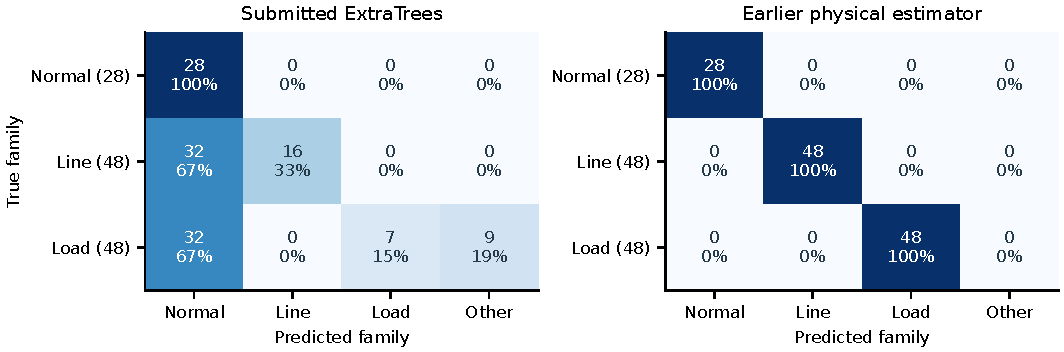
\includegraphics[width=.96\textwidth]{figures/generated/historical_transfer_confusion.pdf}
\caption{Historical development transfer on shared observation windows.
Cells show counts and row percentages. All out-of-scope predictions are
retained as ``Other''; the submitted system's nine such predictions were
the unknown-event label. This is a family matrix, not a localization
matrix. The physical comparator is an earlier estimator, not the final
continuous bank. The 96 event realizations reuse 36 physical event
trajectories; the normal windows come from six physical trajectories.}
\label{fig:historical-transfer}\end{figure*}

This comparison exposes a transfer failure of the delivered system on
the later simulator's load/line catalog. It does not show an official
hackathon-score improvement. The submitted model retains its broader
training domain and 30-s window rule, whereas the physical estimator
knows the simulator and its 12 candidate origins. These were development
cases, and the comparison permits both methods the same window endpoint.
The next study therefore uses separately trained causal ExtraTrees
comparators, successive events and a new frozen cohort. Its results must
be read as a second experiment, not as more independent repetitions of
the perfect development score.


\subsection{Following Successive Events Through Recovery}

The example in Fig.~\ref{fig:narrative-rolling} follows six physical
interventions without restarting the network. With matched R/X, all six
sources are identified before their OFF times. Under a network change
outside the bank, an extra bus-20 diagnosis precedes the real bus-31 load;
bus 31 is then diagnosed only after its physical restoration. The lower
panel shows the mechanism visible to the method: active bus-31 mass rises
late in the mismatched record. This is one development trajectory, not a
performance estimate.

\begin{figure}[t]\centering
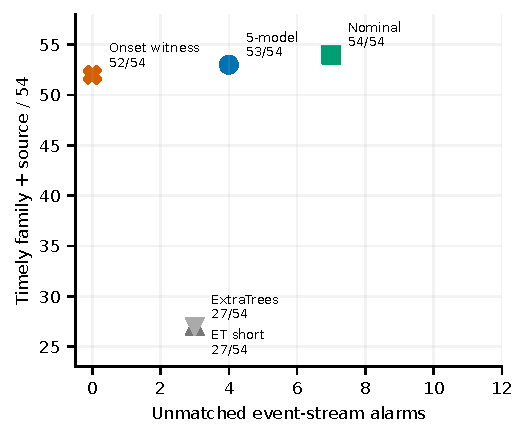
\includegraphics[width=\columnwidth]{figures/generated/narrative_tradeoff.pdf}
\caption{Development decision trade-off on 18 interventions replayed under three R/X settings. A stricter onset witness eliminates extra alarms but misses a true bus-16 load. The 54 plotted realizations share physical parents. These controls were not selected using the later sealed evaluation.}
\label{fig:narrative-tradeoff}\end{figure}

The development controls also show that deleting alarms is easy if true
events may be lost (Fig.~\ref{fig:narrative-tradeoff}). The stricter onset
witness has no extras but loses a real bus-16 intervention. The frozen
five-model procedure was therefore evaluated with its original publication
rule; no rule was revised from the sealed outcomes.

\begin{figure*}[t]\centering
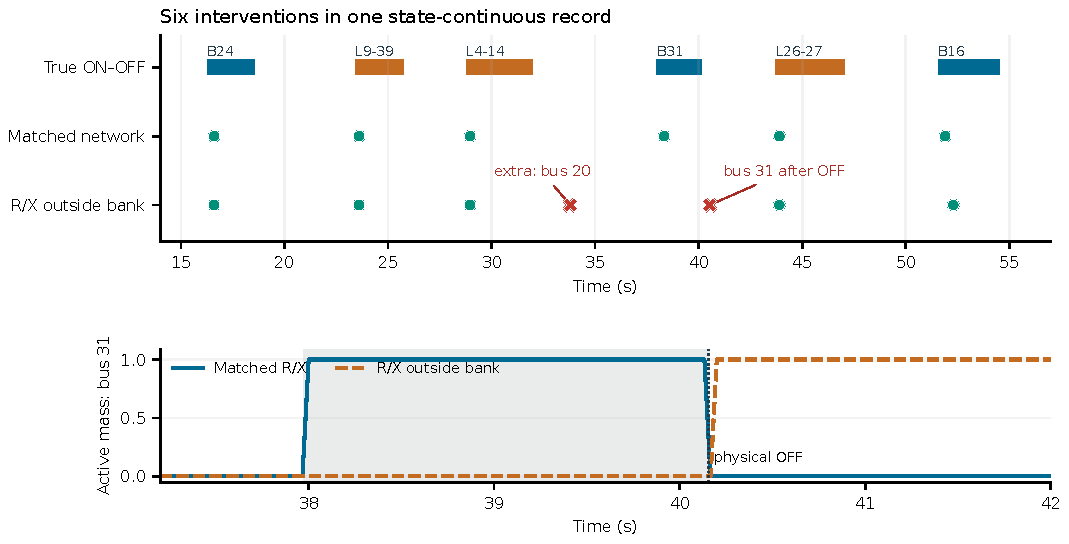
\includegraphics[width=.92\textwidth]{figures/generated/reader_episode_story.pdf}
\caption{One development sequence. Bars show reserved physical ON--OFF truth;
circles are correct diagnoses emitted before OFF; crosses mark an extra
bus-20 alarm and a bus-31 diagnosis emitted after OFF. Both lower decision
rows use the same physical bank under different R/X conditions. The lower
panel shows approximate active mass for bus 31: with R/X outside the bank,
the correct explanation becomes dominant only after restoration. Truth is
shown retrospectively and never enters inference.}
\label{fig:narrative-rolling}\end{figure*}

\subsection{Comparison With a Simpler Physical Procedure}
An earlier development control uses the same nominal physical and PMU
operators, one retained state and a short generalized likelihood-ratio
search. With a common six-report publication clock, it obtains
\SSSimpleTimely{}/\SSSimpleTotal{} timely decisions and
\SSSimpleExtras{} extras; the history mixture obtains
\SSMixTimely{}/\SSMixTotal{} with \SSMixExtras{}. This is an executed
physical comparator, separate from the later confirmatory cohort.
Different search, severity treatment and score semantics prevent it from
being a pure Bayes or memory ablation. Its equations and full table are
included in the supplement.

% Allow following text to fill the column while the full-width history figure floats.
\subsection{Independent Evaluation: Timely Attribution and Alarm Cost}
\label{sec:c01-results}

The five-model bank makes \COneMixTimely{}/\COneMixTotal{} timely
family-and-source decisions with \COneMixExtras{} unmatched alarms on
event records, and its nominal counterpart \COneNomTimely{}/\COneNomTotal{}
with \COneNomExtras{}. These are paired replays of 108 interventions in 18
physical parents, not 648 independent events. On the 72 normal records
(42{,}336\,s, 11.8\,h of monitored time per method) neither bank raises an
alarm, which bounds the normal false-alarm rate below 0.26 per hour at 95\%
confidence (Poisson). Every matched diagnosis emitted before OFF names the
correct family and source; the timely misses are late or absent
diagnoses. Table~\ref{tab:c01-direct} and Fig.~\ref{fig:c01-main} give the
family split.

\begin{table}[t]\centering\small
\caption{Held-out continuous-stream decisions. Each family has 324 replays
of 54 distinct interventions; extras are unmatched alarms on event records.
The ExtraTrees adapters keep their original operating points.}
\label{tab:c01-direct}
\begin{tabular}{@{}lrrr@{}}\toprule
Method & Load & Line & Extras\\\midrule
Physical bank & \ReaderPhysicalLoad/324 & \ReaderPhysicalLine/324 & \COneMixExtras\\
Nominal bank & \ReaderNominalLoad/324 & \ReaderNominalLine/324 & \COneNomExtras\\
ExtraTrees & \ReaderETLoad/324 & \ReaderETLine/324 & \COneETExtras\\
ExtraTrees short & \ReaderETShortLoad/324 & \ReaderETShortLine/324 & \ReaderETShortExtras\\\bottomrule
\end{tabular}\end{table}

\begin{figure*}[t]\centering
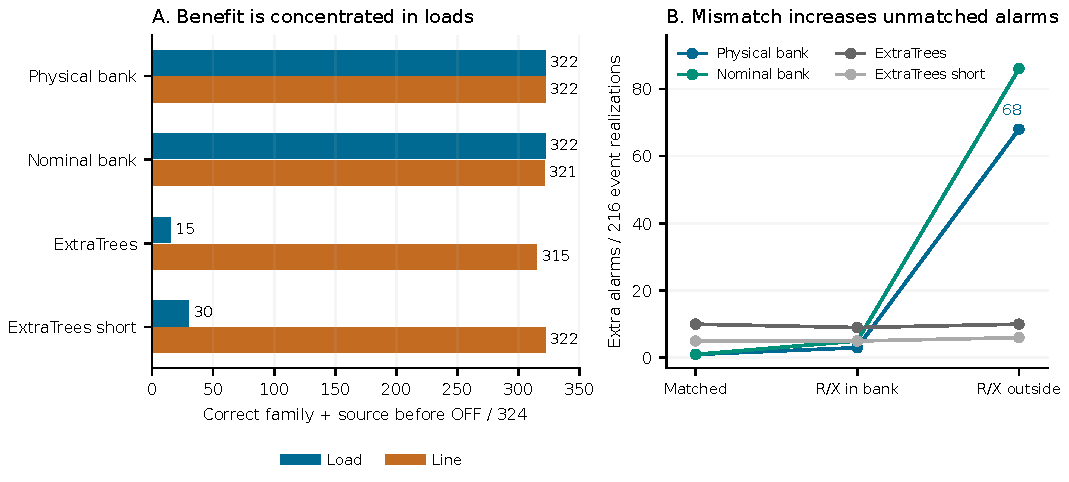
\includegraphics[width=.91\textwidth]{figures/generated/reader_c01_tradeoff.pdf}
\caption{Held-out continuous evaluation. (A) Timely correct family and source
by event family, with 324 paired replays per family. (B) Unmatched alarms on
event records for the two noise levels of each R/X condition (216 event
replays per condition). Each method keeps its own publication rule.}
\label{fig:c01-main}\end{figure*}

The extra alarms concentrate where the network model is wrong: 68 of the
72 occur when the true R/X perturbation lies outside the five-model bank,
68 alarms in 1.08\,h of out-of-bank monitored event-record time (about 63
per hour), against four in the other four strata together. Out-of-bank mismatch also produces the only
four timely misses. The supplement gives the paired parent-cluster
intervals; the physical bank's median alarm delay is about 0.27\,s in the
matched and in-bank conditions, comparable to the learned adapters
(0.19--0.30\,s).

We compare these delays retrospectively with Prediction~1. For the nominal bank on matched networks,
line alarms arrive after a median \RevObsLineDelay\,s, at the six-report
confirmation floor of \RevPredAlarmDelay\,s less the sub-report onset
phase, and doubling the noise leaves them unchanged. Load alarms arrive
after \RevObsLoadDelay\,s, again unchanged by doubled noise but about
\RevLoadExcessReports{} reports after the nominal signature reference crossing. Line delays are
consistent with the publication floor, while load delays exceed that
model-based reference.
The two ExtraTrees adapters recover lines (\ReaderETLine{} and
\ReaderETShortLine{} of 324) but few loads (\ReaderETLoad{} and
\ReaderETShortLoad{}). The diagnosis-time distributions in the supplement show that this is a
coverage failure: every load diagnosis the adapters do emit before OFF is
correct, but most load interventions receive none. A per-report audit on
four further matched records (12 load and 12 line interventions,
1{,}245 and 1{,}143 in-event reports) locates the failure before any
publication rule. During every load intervention the reference model's
per-report argmax is the normal class in all reports, and the median of
the largest true-class score is 0.09; during line interventions the true
line wins 96\% of the reports with median peak score 0.93. The short-window
variant ranks the true load first in only 2 of 12 load interventions. The
learned representation thus does not separate 3--14\% load changes from
normal operation, whereas the nominal physical signatures have large separation energies
for the same changes (Fig.~\ref{fig:theory-information}). The same pattern was already present in
their development validation (Section~\ref{sec:narrative-protocol}), so the
comparison shows that the physical bank recovers load interventions that
these particular adapters miss; it is not a test of the best attainable
learned detector at a common alarm budget.
In the persistent-line test, both banks and both adapters identify the
correct line first on all 162 openings. The adapter of Chen \emph{et al.}'s
quickest-change detector identifies 74/162; 66 records stop before the
opening and 22 afterward on a wrong line, and it stops on all 72 paired
normal records (first stop after 2{,}522\,s of cumulative normal exposure,
against 42{,}336\,s monitored without alarm by the other methods). Its
white-injection, quasi-static model does not describe the colored,
dynamically filtered measurements of this plant, so its threshold is far
from its nominal false-alarm rate. We therefore read this result as a test
of transfer under model mismatch, not as a ranking of quickest-change
detection. After the first identification, the two learned adapters raise
\PersistETExtras{} and \PersistShortExtras{} further unmatched alarms on the
same persistent records, against \PersistPhysicalExtras{} for the
physical bank. Stratified tables, failure ledgers, restoration outcomes and
censoring are in the supplement.

Table~\ref{tab:competition-metrics} restates the evaluation in the metrics
prescribed by the competition guide. Per-report detection F1 is 0.91 for
the bank and 0.58--0.64 for the learned adapters, whose precision is higher
because they alarm only on the line interventions. None of the methods
raises an alarm on the normal records. The bank has no trained weights:
its parameters are the network model, the noise model estimated from normal
data, and a few prior and publication constants fixed during
development. The nominal bank processes one
minute of PMU data in 48\,s on one CPU thread.
\begin{table*}[t]\centering\small
\caption{Independent evaluation in the metric vocabulary of the competition guide (648 interventions, 706\,min of normal records, three R/X conditions pooled). Detection is scored per report; Top-$k$ requires the correct family and source among the first $k$ candidates. Run time is per minute of PMU data on one CPU thread.}
\label{tab:competition-metrics}
\begin{tabular}{@{}lrrrrrrrr@{}}\toprule
Method & Precision & Recall & F1 & FA/min & Delay (s) & Top-1 & Top-3 & Run time (s/min)\\\midrule
Physical bank, five R/X models & 0.888 & 0.926 & 0.907 & 0 & 0.20 & 0.995 & 0.995 & 179\\
Physical bank, nominal model & 0.874 & 0.927 & 0.900 & 0 & 0.27 & 0.995 & 0.995 & 48\\
Submitted ExtraTrees & 0.938 & 0.424 & 0.584 & 0 & 0.27 & 0.509 & 0.509 & --\\
Retrained short-window ExtraTrees & 0.944 & 0.483 & 0.639 & 0 & 0.19 & 0.543 & 0.543 & --\\
\bottomrule\end{tabular}\end{table*}


\section{Episode Restoration and Computational Cost}
\label{sec:closure-results}

Restoration timing gives a second view of continuous attribution. Figure~\ref{fig:closure-restoration} shows the signed OFF delay among available associated restorations, alongside intended events without a restoration value. Under the posthoc threshold of more than one 30-Hz report early ($d_{\rm OFF}<-1/30$ s), the physical bank has 0/644 early restorations and the nominal bank 0/643. The reference and short-window ExtraTrees have 52/330 and 26/352, respectively. The corresponding missing-restoration counts are 4, 5, 318 and 296 out of 648 intended event realizations. Missing values include omissions and are not necessarily open episodes. Replays are dependent; this descriptive criterion is not a new confirmatory endpoint and does not isolate the memory component.

\begin{figure}[t]\centering
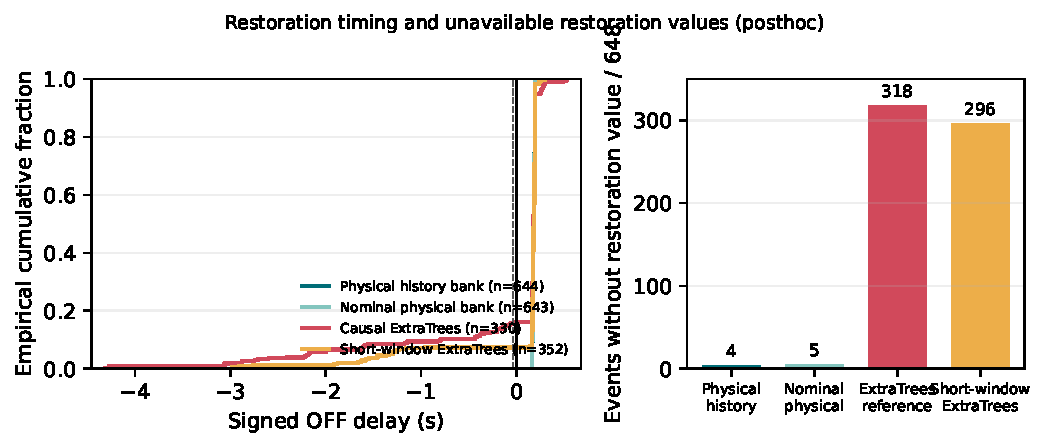
\includegraphics[width=\columnwidth]{figures/generated/closure_restoration.pdf}
\caption{Posthoc restoration timing and events without an associated restoration value. Panel A shows signed OFF delay only where available; the dashed line marks the threshold at one report early. Panel B reports missing restoration values over 648 intended events, including omissions, not a count of episodes open at record end.}
\label{fig:closure-restoration}\end{figure}

Recorded stage timings from the continuous evaluation are summarized in Table~\ref{tab:closure-compute-cost}. For 120-s records, median physical-history inference took 358.7 s across 270 records, compared with 9.5 s for the combined ExtraTrees adapter stage; physical bank construction had a separate 80.1-s median. Dividing total time by 3,601 reports gives amortized averages of 99.6 ms/report for physical inference and 2.6 ms/report for the combined learned stage. These totals include full-record work and do not measure per-report latency. The physical stage is slower in this recorded implementation and does not support a real-time claim. Timers span mixed stages from the evaluation and concurrency; memory use and frame-level latency were not recorded. The 600-s normal controls are summarized separately in the machine-readable cost file.

\begin{table}[t]\centering\footnotesize\setlength{\tabcolsep}{2pt}
\caption{Posthoc description of episode restoration in the continuous evaluation. Early counts restorations with $d_{\mathrm{OFF}}<-1/30$ s (more than one report early); Early (\%) divides by Available. Missing counts absent restoration values out of 648 intended events, including omissions and not necessarily open episodes. Replays are dependent; no significance test is implied.}
\label{tab:closure-restoration}
\begin{tabular}{@{}lrrrr@{}}\toprule
Method & Available & Early & Missing & Early (\%) \\\midrule
Physical bank & 644 & 0 & 4 & 0.0\% \\
Nominal bank & 643 & 0 & 5 & 0.0\% \\
ExtraTrees reference & 330 & 52 & 318 & 15.8\% \\
ExtraTrees short & 352 & 26 & 296 & 7.4\% \\
\bottomrule\end{tabular}\end{table}

\begin{table}[t]\centering\small\setlength{\tabcolsep}{3pt}
\caption{Recorded stage times from the continuous evaluation on 120-s records. Medians and ranges summarize full-record stages; the per-report column is a median-total divided by 3,601 reports and is amortized, not frame latency. Stages were recorded in a campaign with one BLAS and one Julia thread; memory and per-report latency were not recorded. This descriptive table does not establish real-time operation or a speedup under matched implementation conditions.}
\label{tab:closure-compute-cost}
\begin{tabular}{@{}lrrr@{}}\toprule
Stage & Median (s) & Range (s) & ms/report$^\dagger$ \\\midrule
Bank build & 80.1 & 62.0--309.7 & 22.2 \\
History inference & 358.7 & 218.2--2641.1 & 99.6 \\
ExtraTrees (both) & 9.5 & 6.7--50.5 & 2.6 \\
Chen detector & 1.3 & 0.9--10.6 & 0.4 \\
\bottomrule\end{tabular}\end{table}


\subsection{Separating Severity Scoring From State Continuity}
\label{sec:component-study}

The continuous comparison evaluates complete procedures. To distinguish
two mechanisms within the physical bank, we fixed a subsequent $2\times2$
study: marginal amplitude evidence versus a bounded profile score, and
physical-state carry versus removal at inferred closure. The five network
models, observations, startup fits, operators, proposal rules and
publication thresholds are common to all four arms. Identical thresholds
do not imply identical false-alarm rates; both coverage and alarm counts
must be measured.

For one load history and amplitude interval $[l,u]$, write its accumulated
conditional log likelihood as
\begin{equation}
 \ell_k(a)=c_k+b_k a-\tfrac12 G_k a^2.
 \label{eq:ablation-quadratic}
\end{equation}
The original score uses $B_k=\log\int_l^u
\exp(\ell_k(a)-c_k)p(a)\,da$ with the existing truncated Gaussian prior.
The alternative uses
\begin{equation}
 \widehat a_k=\operatorname{clip}_{[l,u]}(b_k/G_k),\qquad
 Q_k=b_k\widehat a_k-\tfrac12G_k\widehat a_k^2,
 \label{eq:ablation-profile}
\end{equation}
with the constant-likelihood case treated separately. Each report adds
$B_k-B_{k-1}$ or $Q_k-Q_{k-1}$, so a rolling replay does not repeatedly
add the same suffix evidence. The conditional Gaussian amplitude/state
updates remain unchanged. Profile weights are normalized scores, not
posterior probabilities. This intervention tests the amplitude-scoring
choice, rather than removing every Bayesian calculation.
The existing Gaussian sufficient statistics supply
$G_k=v_k^{-1}-v_0^{-1}$ and $b_k=\mu_k/v_k$, removing the computational
prior precision before profiling. Fixed line-opening amplitudes and the
prior weights of amplitude intervals are unchanged.

At an internally inferred closure, the carry arm retains the projected
augmented state. The reset arm sets its 114 estimated physical-state
deviations to zero and retains instrumental/discrepancy coordinates,
covariance regime and network-model weights. This is an estimator
ablation: every observed record comes from the same continuous physical
trajectory. It does not test removal of all temporal information.

The protocol uses all 18 matched-network continuous parents at the
original noise level, plus the first three normal and persistent-line
parents by identifier. It was fixed before ablation outcomes, but the
underlying records had already been examined. Results are therefore a
posthoc mechanism study, with paired intervals over physical parents,
not a new independent confirmation.

\subsection{Effect of Preserving the Physical State}
\label{sec:controlled-ablation}
\begin{table*}[t]\centering\scriptsize
\caption{Controlled amplitude-score and physical-state-carry ablation. Same five-model bank and publication rules. All 18 continuous parents (108 events) are retained. Normal controls comprise three 600-s records with 588 s evaluated exposure each (1,764 s total; startup excluded). Delay is conditional on emitted matched diagnoses and must be read with the no-timely-diagnosis count.}
\label{tab:a01}
\begin{tabular}{lrrrrrr}\toprule
Procedure & Timely & Extras & Normal FA & False restorations & No timely & Delay (s)\\\midrule
Marginal + carry & 108/108 & 1 & 0/1,764 s & 1 & 0/108 & 0.267\\
Profile + carry & 108/108 & 1 & 0/1,764 s & 1 & 0/108 & 0.267\\
Marginal + reset & 75/108 & 166 & 0/1,764 s & 130 & 33/108 & 0.337\\
Profile + reset & 75/108 & 166 & 0/1,764 s & 130 & 33/108 & 0.337\\
\bottomrule\end{tabular}\end{table*}

\begin{figure*}[t]\centering
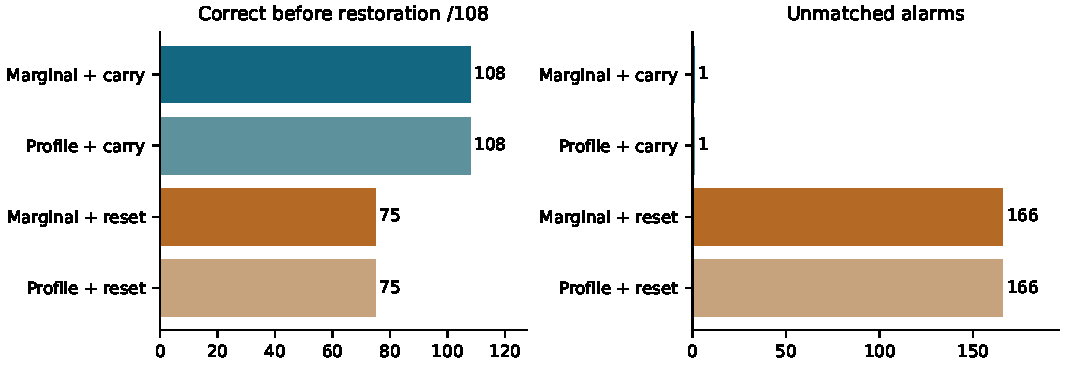
\includegraphics[width=.92\textwidth]{figures/generated/ablation_a01.pdf}
\caption{Severity-scoring and state-carry study on identical observations and five-model banks. The 108 interventions belong to 18 continuous trajectories. Thresholds are fixed, so the alarm rate may differ between arms.}\label{fig:a01}\end{figure*}
The nominal bank and the continuous GLR both carry physical state.
Their primary comparison therefore cannot identify the effect of resetting
it. In the fixed-threshold component study, resetting only the physical
coordinates reduced timely attribution from 108/108 to 75/108 and increased
unmatched alarms from 1 to 166 (Table~\ref{tab:a01} and Fig.~\ref{fig:a01}).
Marginal and profile severity scores gave the same outcomes within each
state treatment. The simulation itself evolves continuously in all arms.

\begin{figure}[t]\centering
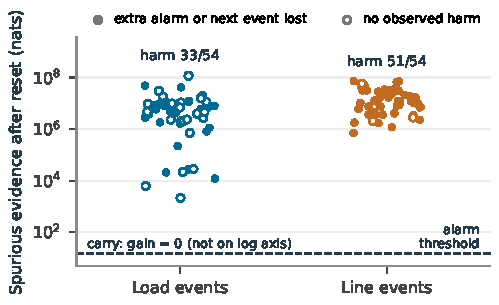
\includegraphics[width=\columnwidth]{figures/generated/theory_reset_cost.pdf}
\caption{Retrospective profiled energy gain after a state reset, \eqref{eq:reset-bias}, for the 108 interventions of the controlled study. Filled: an extra alarm in the following gap or a lost timely attribution of the next intervention; open: neither. The dashed line is the idealized score reference, not the publication threshold. Under matched noise-free continuation, carrying the state gives no positive gain over the null.}
\label{fig:theory-reset}\end{figure}

Fig.~\ref{fig:theory-reset} compares this outcome with the retrospective reset diagnostic. The
profiled energy gain exceeds $\lambda^\star$ after every intervention, by at
least two and up to seven orders of magnitude, and the reset arm is harmed
after \RevResetHarm{} of the \RevResetEvents{} interventions: an extra alarm
in the following gap or a lost timely attribution of the next one. Harm
occurs after \RevResetHarmLine{} line events and
\RevResetHarmLoad{} load events. The bus-31 events carry the smallest
profiled gain and are harmed after three of seven. The diagnostic shows
that reset leaves a residual that event candidates can explain. Its
magnitude alone does not determine the observed outcome: episode handling
and publication rules also matter. These are within-simulator contrasts at the
original thresholds; the two scores are compared at equal thresholds, not
at equal alarm rates.

\section{Discussion and Limits}
\label{sec:discussion}

\subsection{Physical-State Continuity as a Design Choice}
The strongest controlled result is the state-carry contrast. Physical OFF
restores an input or branch, while the machines retain their state.
Removing those estimated deviations at inferred closure substantially
worsens decisions on the same records. Marginal and bounded-profile
severity scores tie on the measured endpoints; both retain conditional
state estimation. This supports recovery-consistent prediction, without
showing that Bayesian marginalization is necessary for those endpoints.

The history bank gives a concrete way to represent the remaining response
and compare it with later interventions. Its complete operational behavior
is measured, but the reset control is deliberately severe. A continuous
physical observer without explicit recovery-history competition could
retain the same consistency. The open-development single-state GLR comparison gives preliminary
evidence against one such alternative, with different search and score
semantics. Independent validation under matched information and a common
calibration contract remains the key unresolved mechanism test.

\subsection{What Improved Relative to the Learned Reference}
The improvement concerns timely coverage of load sources under this
known-catalog simulator contract. Line coverage is comparable to the
short-window learned adapter. The physical method also issues more extra
alarms under network mismatch. The result is therefore a coverage--alarm
trade-off at fixed thresholds, rather than dominance at equal alarm rates
or a higher official hackathon score. Engineering physical features is
useful in the historical learned route; the physical bank additionally
computes how each candidate intervention should affect remote PMUs.
These routes have different access to source responses and training data.

A matched architecture comparison requires a physical continuous-state
control and a history bank with the same operators, together with a learned
baseline trained on the permitted catalog. Operating points must be chosen
on separate calibration records before a new test. The present comparison
preserves the frozen adapters and their failures. The two learned models
already saw all candidate classes during their earlier training; their
misses cannot be attributed solely to missing source labels or to an
unexamined scalar threshold.

\subsection{Model Correspondence and Measurement Scope}
The nonlinear generator and local predictors share the same research
plant family. Switched dynamics, nonlinear responses, noise and out-of-bank
R/X challenge the inverse model, but do not remove this shared-model
advantage. Independent dynamic-model or cross-simulator transfer remains
untested. All nine load and nine line candidates were inherited from
method development before the independent draw; they are a declared
catalog, not a representative sample of all 39 buses or all event families.

The eight-PMU terminal map is a research measurement hypothesis. BUS5
retains the provisional 5--6 assignment, and BUS39 current angle is excluded.
The synchronized channel grouping includes remote current terminals, so
it does not certify an installation of eight colocated voltage/current
PMUs. The observation model retains each terminal's actual location;
remote voltage--current products are power proxies.
The generator applies temporal and cross-PMU noise structure within each
signal family, but does not apply its archived cross-family factor
covariance. Frequency/ROCOF noise is added after phase estimation.
The experiment therefore does not validate a complete physical PMU noise
model, a producer's CT placement or exact reproduction of the historical
reference record. It also assumes an event-free startup and available PMUs.

\subsection{Approximation and Decision Uncertainty}
History pruning, shared regime covariances, plug-in startup estimates and
state-mean compression make the bank approximate. Its masses are
attribution weights under those approximations, not validated confidence
levels. The supplementary numerical checks verify the severity integral,
partition identity and conditional-state algebra under their local models.
Calibration of the nonlinear stream additionally requires pre-update
innovation diagnostics, interval coverage and sensitivity to pruning and
state compression. Existing instrumental whitening and latent AR states
address distinct components of dependence; their presence alone does not
establish predictive adequacy. Discarded mass is recorded by the
implementation, while a calibrated reliability and bank-size study remains
open.
Response fidelity and source discrimination also differ: sources may
remain close after fitting severity and context. The supplementary
context-signature and recovery-geometry controls preserve their null
source-decision results and do not supply an online identifiability
certificate. A useful extension would test whether a causal separation
margin predicts errors and delays before using it to justify abstention.

The measured research implementation runs below the input cadence.
Decision timestamps, computation delay and queueing must remain separate.
These results support further diagnostic development, rather than
protection or control deployment.

\section{Conclusion}
\label{sec:conclusion}

A restored load or line can leave a transient that resembles a new
intervention. The proposed bank predicts that transient from the carried
state and evaluates new source hypotheses against it. At a common
calibration target, the bank correctly attributed \RecBankTimely{}
interventions before restoration, compared with \RecGlrTimely{} for a
continuous GLR and \RecTreesTimely{} for ExtraTrees. During event records,
the three procedures emitted \RecBankExtras{}, \RecGlrExtras{} and
\RecTreesExtras{} unmatched alarms, respectively.

Resetting the physical state at inferred closure reduced coverage at fixed
thresholds. The difference between the complete procedures leaves open
how much explicit history retention adds beyond carrying state.
The evidence covers nonoverlapping load and line events from a fixed
catalog in one simulator family. Most unmatched alarms in the separate network-mismatch test occurred
under perturbations outside the five-model set. Independent per-PMU noise
reduced load attribution.


\FloatBarrier
\bibliographystyle{IEEEtran}
\bibliography{references}
% Public-source biographies authorized by the user on 31 October 2026.
% Evidence: docs/submission_successor_20261031/AUTHOR_PUBLIC_SOURCES.json.
% Keep author order. Verified institutional portrait sources are documented in
% figures/author_photos/PROVENANCE.md. Jorge and Yessica remain without photos
% until an attributable portrait is supplied.

% J2/J3: self-entered ORCID education and Uniandes thesis; no degree-conferral
% date, master's degree, or current university employment is asserted.
\begin{IEEEbiographynophoto}{Jorge Luis Mayorga Taborda}
studied electronic engineering at Universidad de los Andes, Bogot\'a, Colombia. His academic work has addressed distributed control using population dynamics, including applications to urban traffic systems.
\end{IEEEbiographynophoto}

% Y3/Y4: Uniandes thesis and IEEE-deposited publication metadata.
% No degree-conferral claim, current job title, or middle-name addition.
\begin{IEEEbiographynophoto}{Yessica Africano Rodriguez}
carried out undergraduate thesis work on photovoltaic integration at Universidad de los Andes, Bogot\'a, Colombia. Her published research includes co-simulation and stochastic assessment of photovoltaic hosting capacity in distribution systems.
\end{IEEEbiographynophoto}

% M1/M3/M4: Pitt institutional profile. Rank intentionally omitted because
% its contact card says Associate Professor while its narrative says assistant.
\begin{IEEEbiography}[{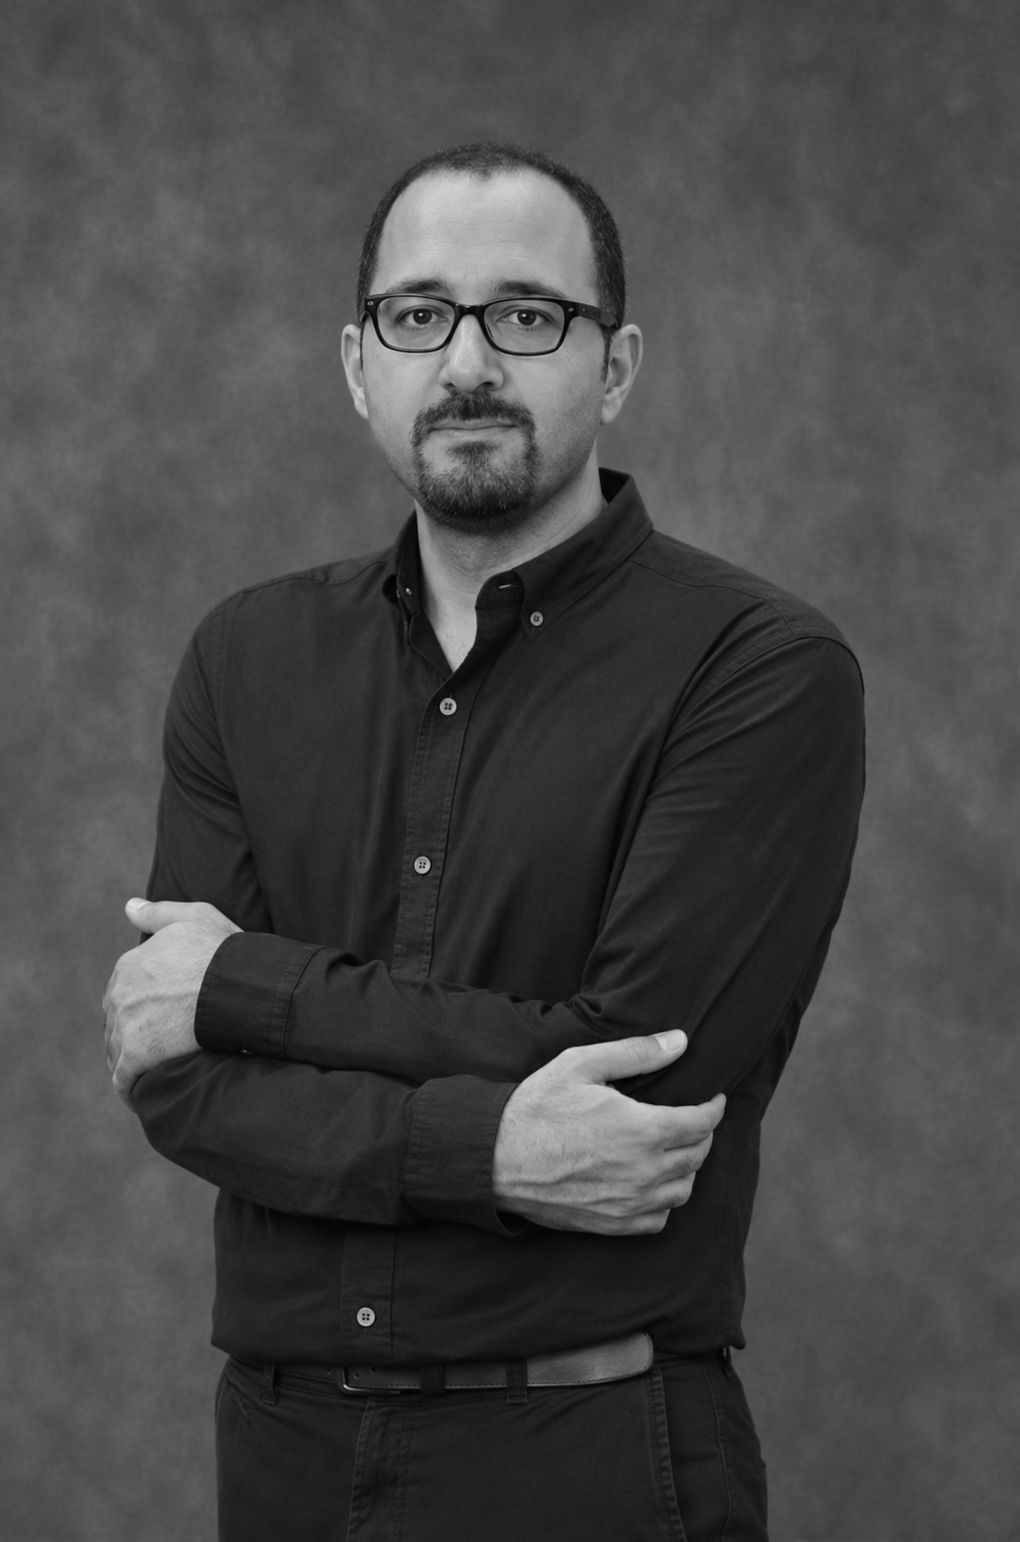
\includegraphics[width=1in,height=1.25in,clip,keepaspectratio]{figures/author_photos/masoud_barati_bw.png}}]{Masoud Barati}
received the Ph.D. degree in electrical engineering from the Illinois Institute of Technology in 2013. He is with the Department of Electrical and Computer Engineering, University of Pittsburgh, Pittsburgh, PA, USA. His research includes mathematical modeling and optimization of electric power systems.
\end{IEEEbiography}

% P1/P2/P3: current GWU faculty page.
\begin{IEEEbiography}[{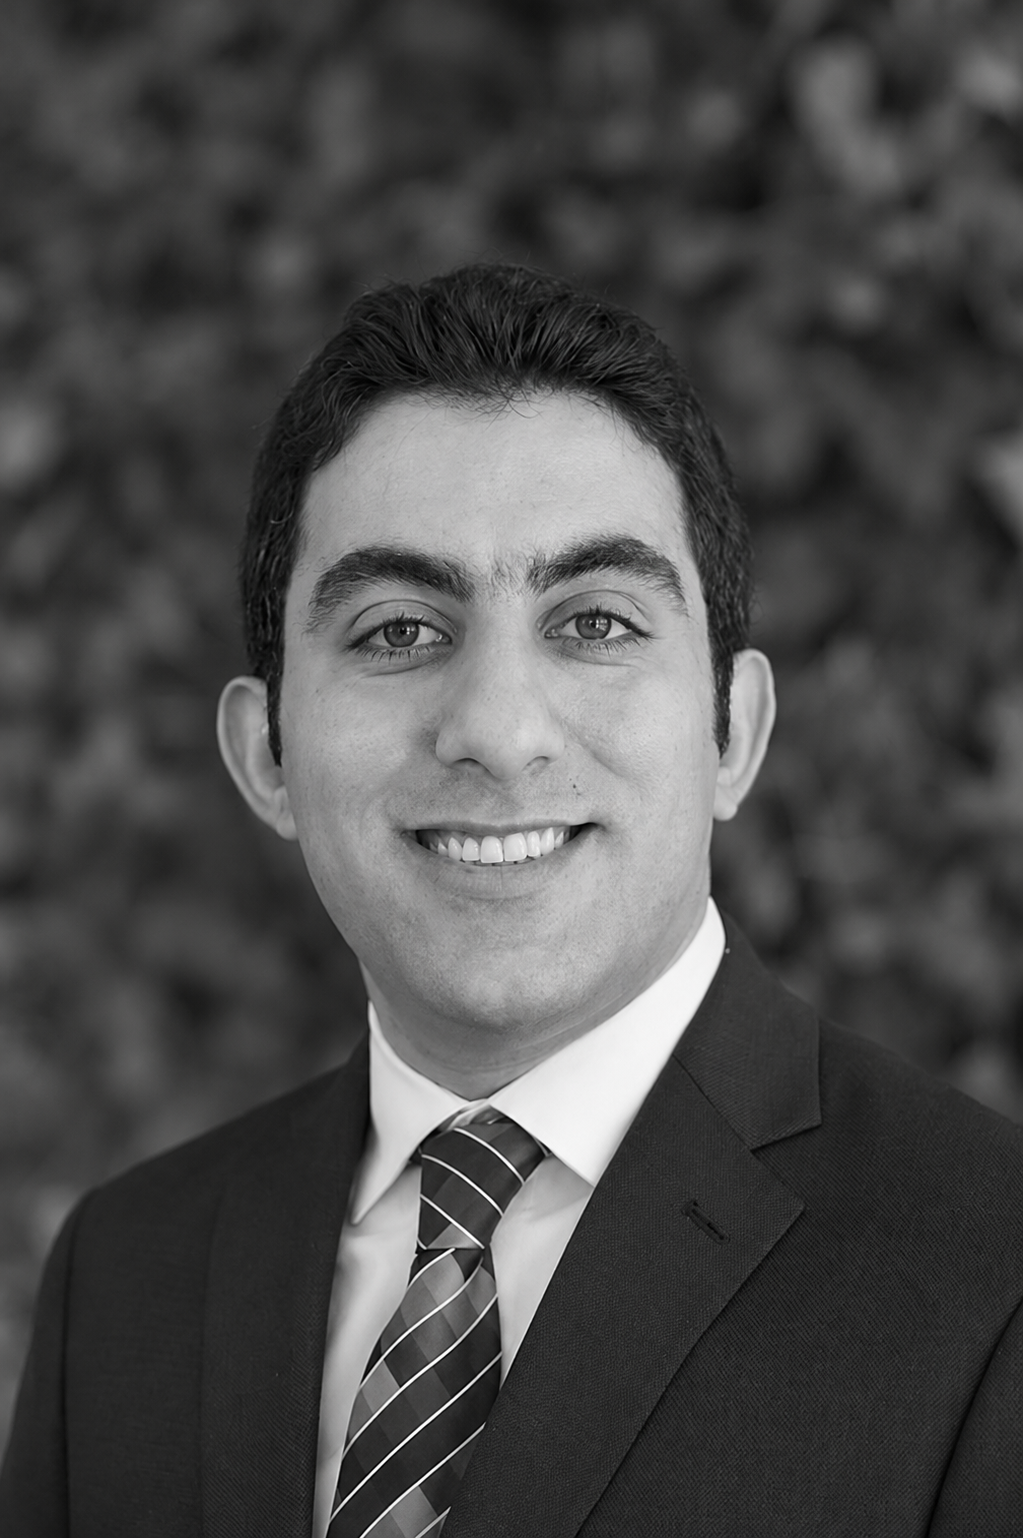
\includegraphics[width=1in,height=1.25in,clip,keepaspectratio]{figures/author_photos/payman_dehghanian_bw.png}}]{Payman Dehghanian}
received the Ph.D. degree from Texas A\&M University in 2017. He is an Associate Professor with the Department of Electrical and Computer Engineering, The George Washington University, Washington, DC, USA. His research includes power-system reliability, resilience, and data-informed decision-making.
\end{IEEEbiography}

% D1/D2/D3: La Sabana institutional profiles; broad institutional degree wording.
\begin{IEEEbiography}[{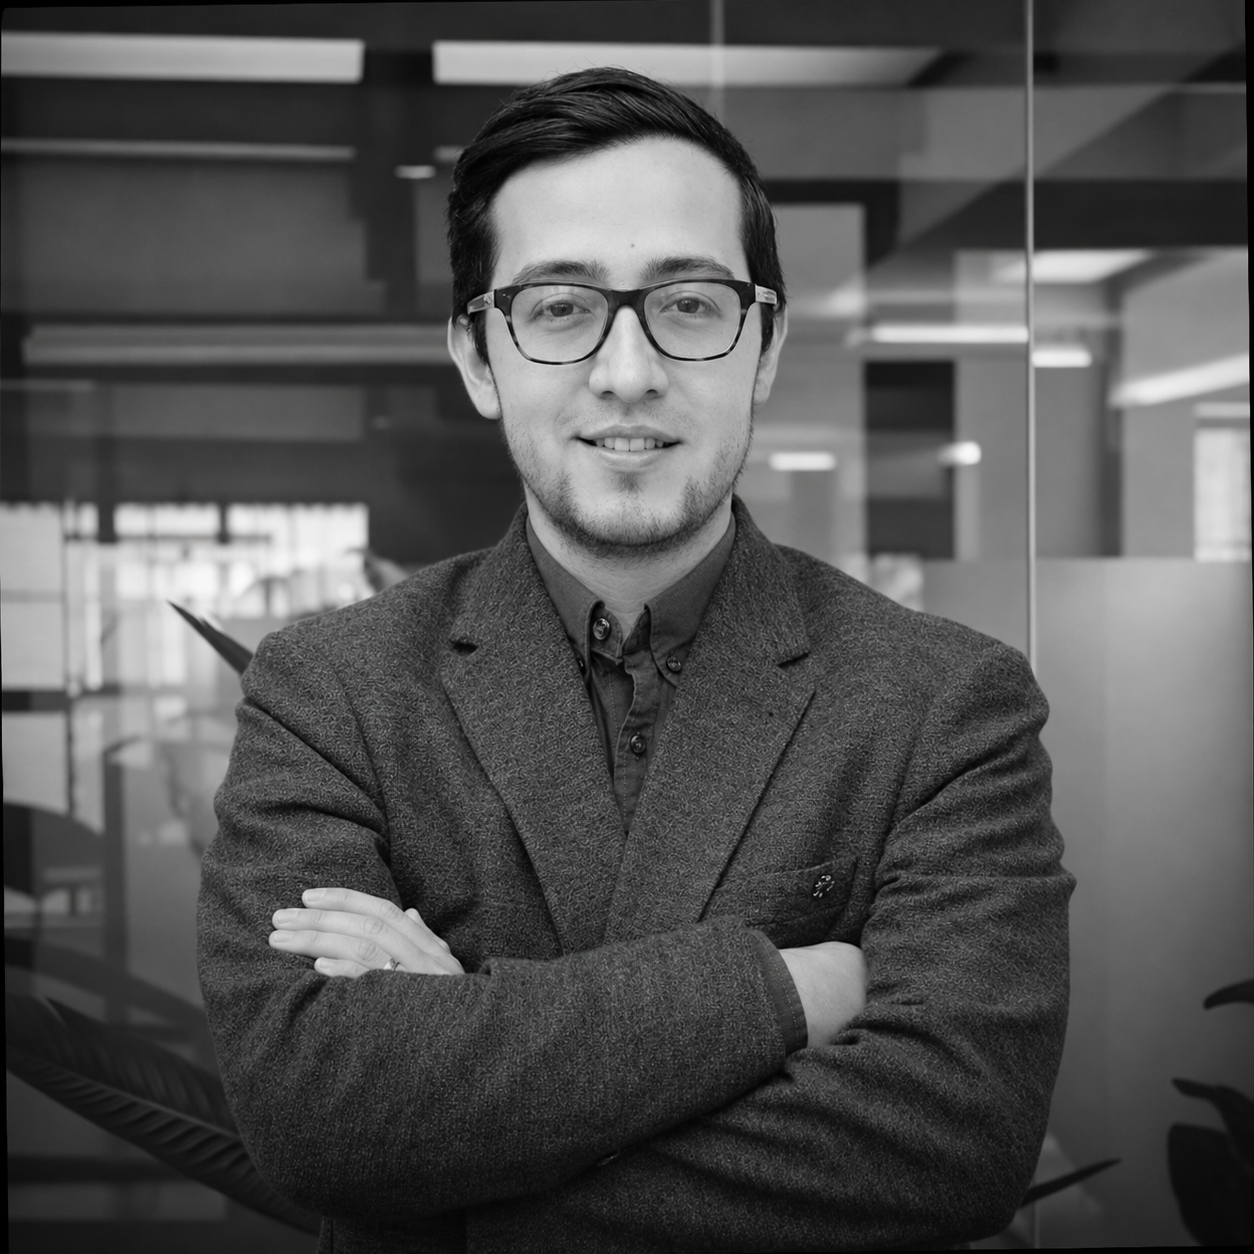
\includegraphics[width=1in,height=1.25in,clip,keepaspectratio]{figures/author_photos/david_celeita_bw.png}}]{David Felipe Celeita Rodr\'iguez}
received the Ph.D. degree in engineering from Universidad de los Andes, Bogot\'a, Colombia. He is an Associate Professor and Director of Outreach and Engagement with the Faculty of Engineering, Universidad de La Sabana, Ch\'ia, Colombia. His research includes power-system protection, fault location, and real-time simulation.
\end{IEEEbiography}

\EOD

\end{document}
